\part{Education}
\label{p:education}
\epigraph{Pass on what you have learned. Strength. Mastery. But weakness, folly, failure also. Yes, failure most of all. The greatest teacher, failure is.}{\textit{Yoda}}

\clearpage
\section*{Introduction}
%(CONTEXT): background for less specialized readers and establish or recalls the importance of the problem
Education in the paved path methodology should be deliberate and keep the developer experience in mind.
The \gls{scw} training platform is a good resource for education in the paved path methodology. 
It provides online training through defensive secure coding exercises in many different programming languages and frameworks, and its gamification and interactivity make it fun and usable.
%
%% (NEED): motivates the audience by stating the difference between the desired and actual situation
%% ==>shortcomings and goal from my perspective
Despite the focus on developers and its many usability features, there is still a significant part of the user base that only follows a minimal amount of training.
Users follow one of the predetermined courses, and it is likely that the pacing of these courses does not fit their needs.
Users get bored due to too much repetition, or frustrated because the content is moving too fast.

%(The TASK) what did I do?
%=> IRT, ITS
I created an \gls{its} by combining psychometric models with techniques from computer science to recommend exercises to each individual at any point in time. 
A customized recommendation like this is more likely to keep the developer engaged and allows meaningful learning to take place.

I start Part~\ref{p:education} by giving an overview of the \gls{scw} training platform, its features, and the different types of exercises in Chapter~\ref{ch:scw}.
I then describe the design of the \gls{its} and explain the used techniques in more detail in Chapter~\ref{ch:its-implementation}.
The last chapter in this part provides an evaluation of the \gls{its} before offering some perspectives that remain future work.

%%(FINDINGS) what did I find?
%\todo[inline]{what did I find?}
%(TODO) The recommendation system was able to predict the learning outcome of challenges in historical data with XX\% accuracy. 
%
%%(CONCLUSION) what does this mean for the need?
%\todo[inline]{what does this mean for the need? --> will there be better engagement? More learning?}
%(TODO) Recommending only challenges with a high probability of a positive learning outcome greatly improves the efficiency of the education.
%It also reduces the mismatch in learning pace and keeps developer engaged longer.
%The \gls{its} also allows us to identify defect exercises, as well as promote new content.
%
%%(PERSPECTIVES) what now?
%%=> integrations
%%=> ecosystem
%There are still opportunities to improve the \gls{its} in the future. 
%The psychometric models allow us to take into account the ability of a user, however, we expect the agility of a user to be important as well.
%It is also possible that recommendations can be improved by taking into account data from other developer tools, such as the issue tracking system, the code repository, and security tools. 
%The current implementation only uses data from the training platform itself.

\chapter{Secure Code Warrior}
\label{ch:scw}
\glsresetall

%CONTEXT
In the paved path methodology, developers should be provided with deliberate, targeted education that keeps the developer experience in mind.
%NEED
This education should be \textit{relevant} to the developers work, \textit{efficient} in achieving their needs, and \textit{usable} to keep them engaged.

%TASK/OBJECT
In this chapter I describe the education provided by the online learning platform created by \gls{scw}. 
I assess its potential for use in the paved path methodology and describe shortcomings that require further research.


\summarybox{
%FINDINGS
The \gls{scw} training platform provides training to hundreds of thousands of developers from reputable customers.
It provides defensive exercises in a gamified and engaging way and offers a wide variety of programming languages and frameworks. 
%CONCLUSION
It is suitable to be used in the paved path methodology as it is \textit{relevant} and \textit{usable}.
However, there is room for improvement when it comes to the \textit{efficiency} of the training.
All users, regardless of skill level, are presented challenges of the same difficulty.
This leads to boredom or frustration for some users and might cause them to disengage from the training.}

\section{The company}
The company was co-founded by Pieter Danhieux and Matias Madou Ph.D., two alumni of Ghent University and both globally recognized security experts.
During their international careers, both founders noticed that the focus in industry is too often on remediation rather than prevention of \glspl{security problem} in software.
Their vision is not to make a security expert out of every developer, but to empower them to become the first line of defence in the organisation.
The company provides education and tools to improve secure coding skills of developers.
Both the online training platform and their IDE based security tool can be deployed to support a paved path methodology as described in this book.

Since its start in 2015, more than 240 customers from 32 countries around the world use \gls{scw} products to improve the secure coding skills within their development teams.
\Gls{scw} focuses on large companies with lots of developers. Most customers are active in banking, finance, government, aviation, or telecommunications. Some notable customers are:

\begin{itemize}
\setlength\itemsep{0em}
    \item Coupang: the largest online retailer in South Korea
    \item 19 of the top 100 global banks
    \item \gls{bbc}: the largest broadcaster in the world
    \item 2 of the world's largest telecommunications providers
    \item 2 of the top US credit card processors
    \item Zoom: one of the largest communication technology companies
\end{itemize}

\section{The training platform}

The training platform provides an interactive and gamified way to learn secure coding concepts, and focuses on defensive techniques. 
In the mission control dashboard, shown in Figure~\ref{fig:mission}, developers are tasked with defending an application from different types of threats originating from all over the world.
The developer is awarded points for completing exercises, and leaderboards are shown to create a competitive environment.
By collecting enough points and spending enough time on the platform, the developer can unlock achievements and gain badges.
All of this progress can be monitored on a metrics dashboard, shown in Figure~\ref{fig:metrics}.
A total of over 100,000 unique developers used the training platform in 2020.

In a survey with 722 developers, 90\% of respondents said they prefer \gls{scw} over traditional classroom learning
and 85\% prefer it over other online learning resources they have tried in the past.
These results are also confirmed by many testimonies, such as the following response on TechValidate\footnote{\url{techvalidate.com/product-research/secure-code-warrior/facts}}. 

\begin{displayquote}
Secure Code Warrior’s use of gamification has helped us emphasize the importance of secure coding in a refreshingly fun and engaging way. \textit{-- Developer at Global 500 Financial Services Company}
\end{displayquote}

\begin{sidewaysfigure}
  \centering
  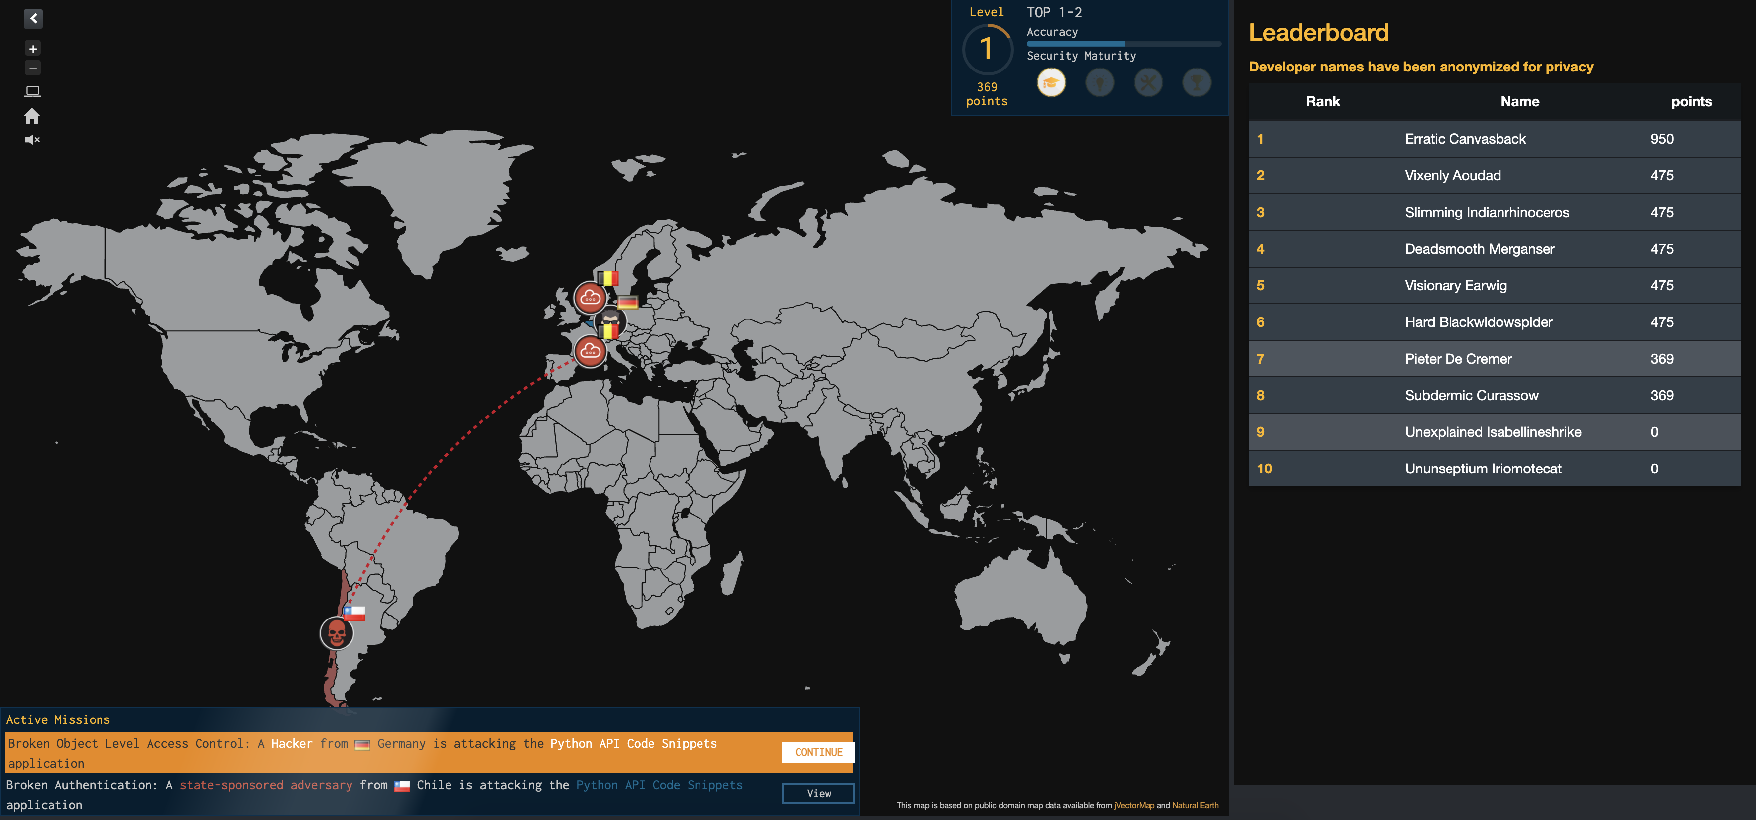
\includegraphics[width=\textwidth]{mission.pdf}
  \caption[SCW mission control dashboard]{The mission control dashboard on the \gls{scw} platform creates a gamified overview of the exercises.}
  \label{fig:mission} 
\end{sidewaysfigure}

\begin{sidewaysfigure}
  \centering
  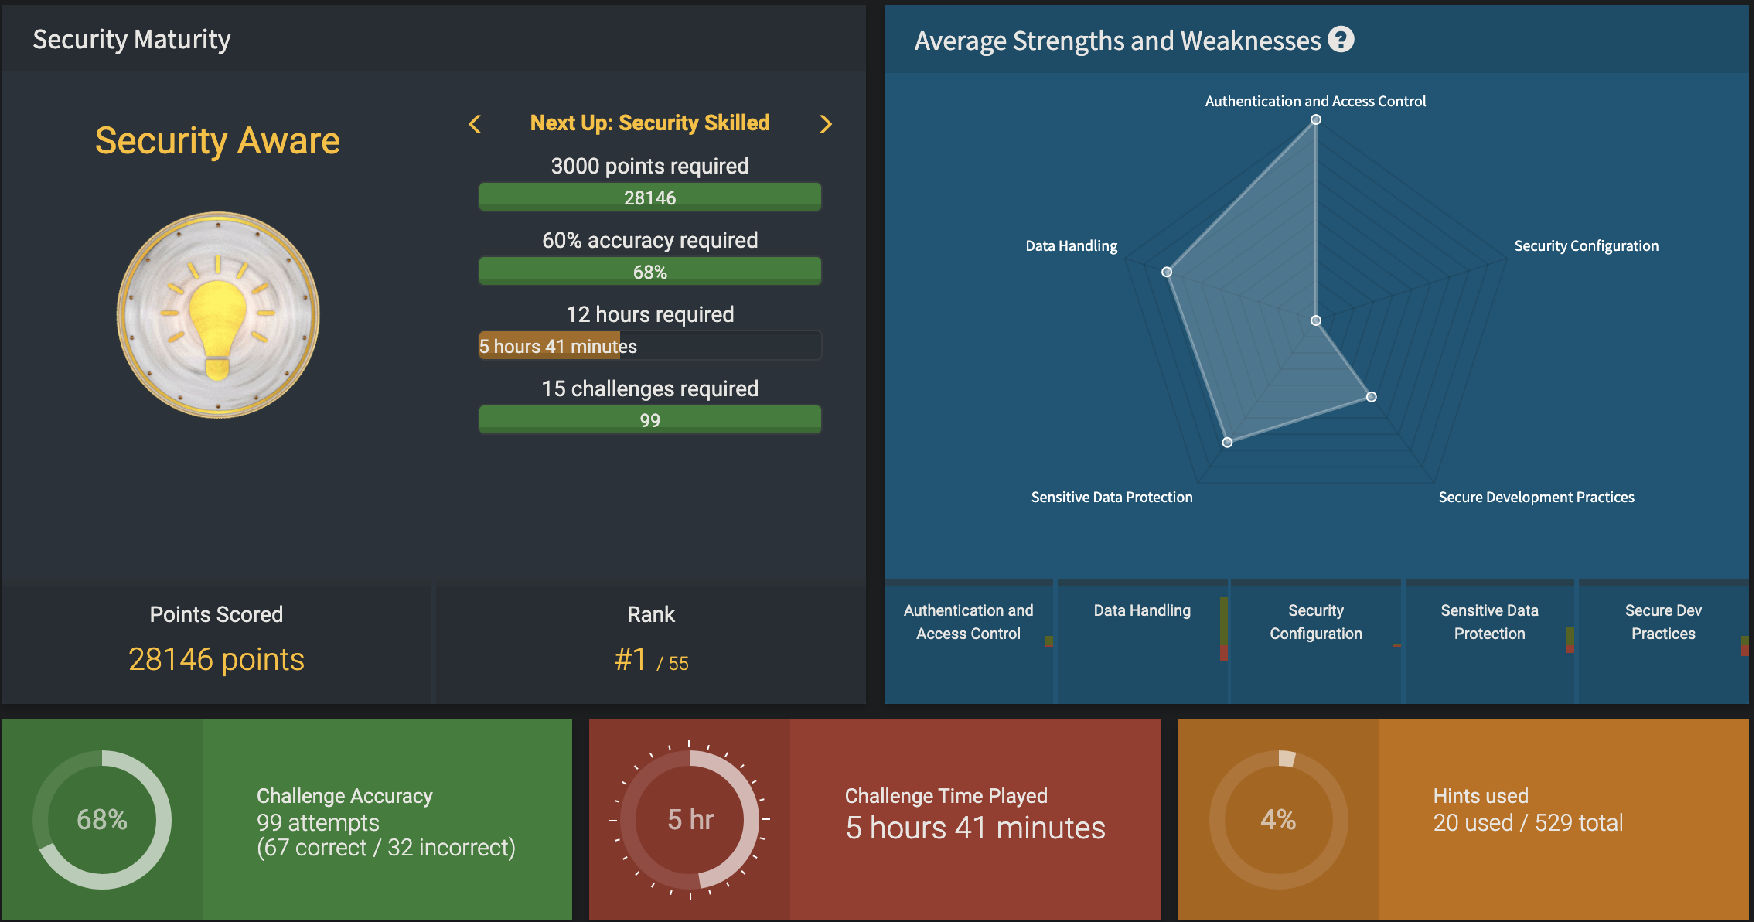
\includegraphics[width=\textwidth]{metrics.pdf}
  \caption[SCW metrics dashboard]{The metrics dashboard on the \gls{scw} platform allows developers to monitor their progress and unlock new badges.}
  \label{fig:metrics} 
\end{sidewaysfigure}

\section{Exercises}
\label{sec:challenges}
Training exercises on the \gls{scw} platform, often called challenges, are most frequently created from a complete and secure software application such as a webstore or a banking application. To create a challenge, a \gls{vulnerability} is introduced into this application on purpose.
The challenge is presented to the users as one of three types of exercises, each assigned a numerical level, an \textit{identify} (L1), \textit{locate} (L2), or \textit{fix} exercise (L3).

Identify exercises (L1) mark the insecure code fragment and provide the developer with a number of \gls{vulnerability} categories. It is up to the developer to identify which of the provided categories best describes the vulnerability present in the code fragment. In Figure~\ref{fig:identify} an identify exercise is shown based on a \gls{sql} injection in a Python web application.

For locate exercises (L2), the category of the vulnerability that is present in the insecure code fragment is given.
The insecure code fragment is marked, as well as several other (secure) code fragments. 
It is up to the developer to locate which code fragment contains the insecurity.
An example of a locate exercise is shown in Figure~\ref{fig:locate} using the same \gls{sql} injection in the same Python web application as the identify exercise in Figure~\ref{fig:identify}.

Fix exercises (L3) show both the insecure code fragment and the category of the inserted vulnerability to the user. 
Four alternatives are shown, with changes made to the insecure code fragment, and sometimes to other parts of the application code as well.
The developer needs to find the most secure alternative among the four options.
A fix exercise is shown in Figure~\ref{fig:fix}, again using the same \gls{sql} injection as before. 
Fix (L3) exercises are often combined with identify (L1) or locate (L2) exercises. 
These challenges then consist of two stages, in the first stage the vulnerability needs to be identified or located, in the second stage the exact same vulnerability needs to be fixed. 
The resulting two-stage challenge is an identify-and-fix (L4 = L1 + L3) or a locate-and-fix (L5 = L2 + L3) challenge.

%\begin{figure}
%\centering
%\begin{subfigure}[b]{\textwidth}
%\sidebysidecaption{0.05\linewidth}{0.95\linewidth}{
%   \caption{}
%   \label{fig:identify}}{
%   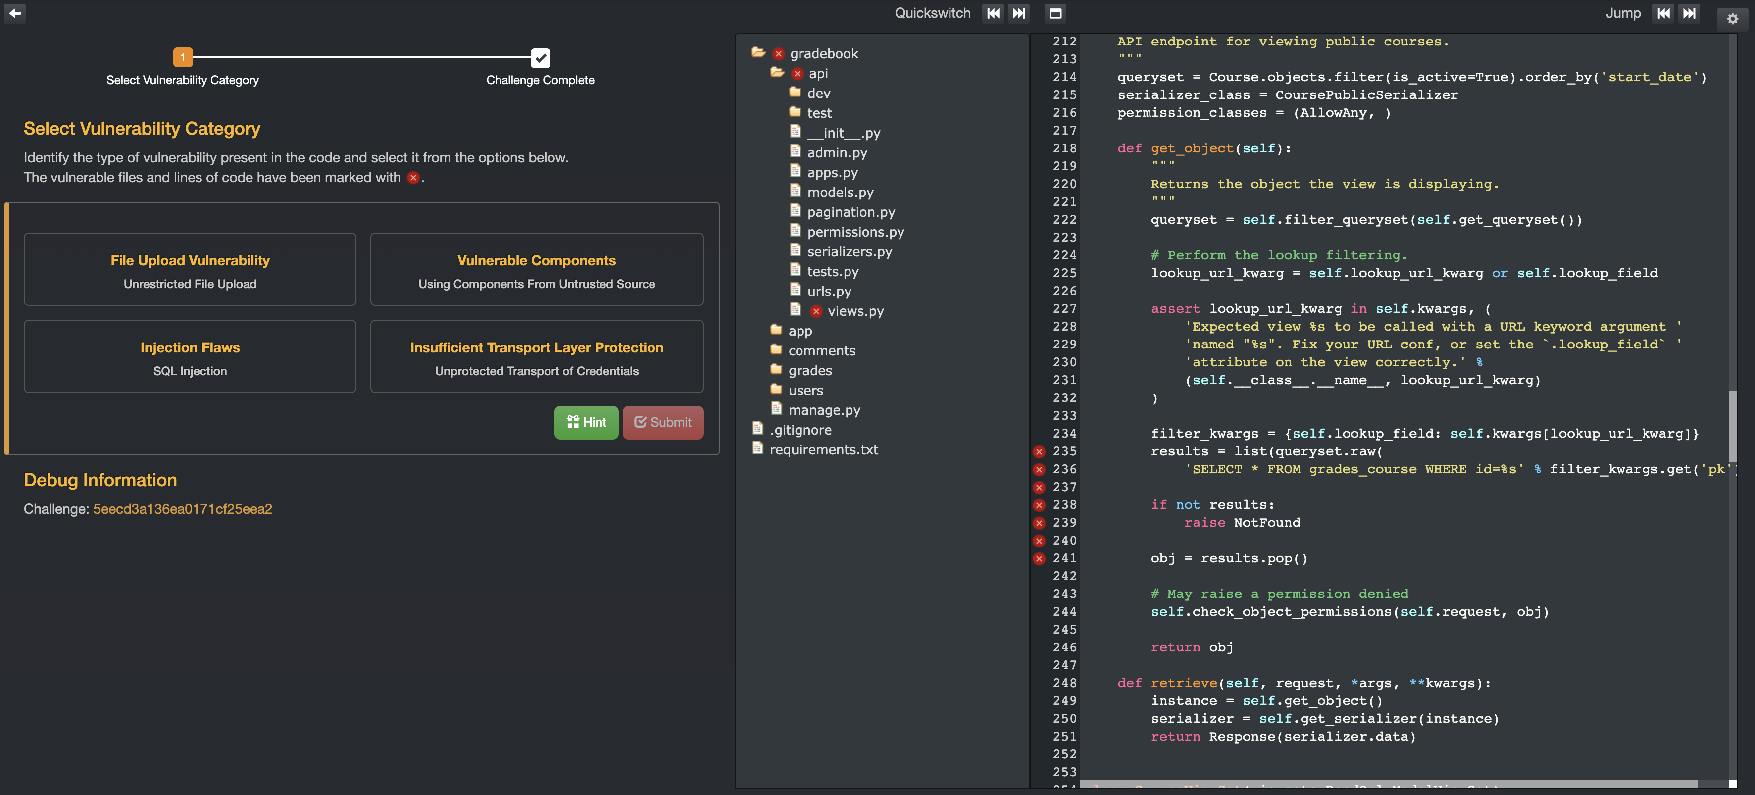
\includegraphics[width=0.95\linewidth]{identify.pdf}}
%\end{subfigure}
%
%\begin{subfigure}[b]{\textwidth}
%\sidebysidecaption{0.05\linewidth}{0.95\linewidth}{
%   \caption{}
%   \label{fig:locate}}{
%   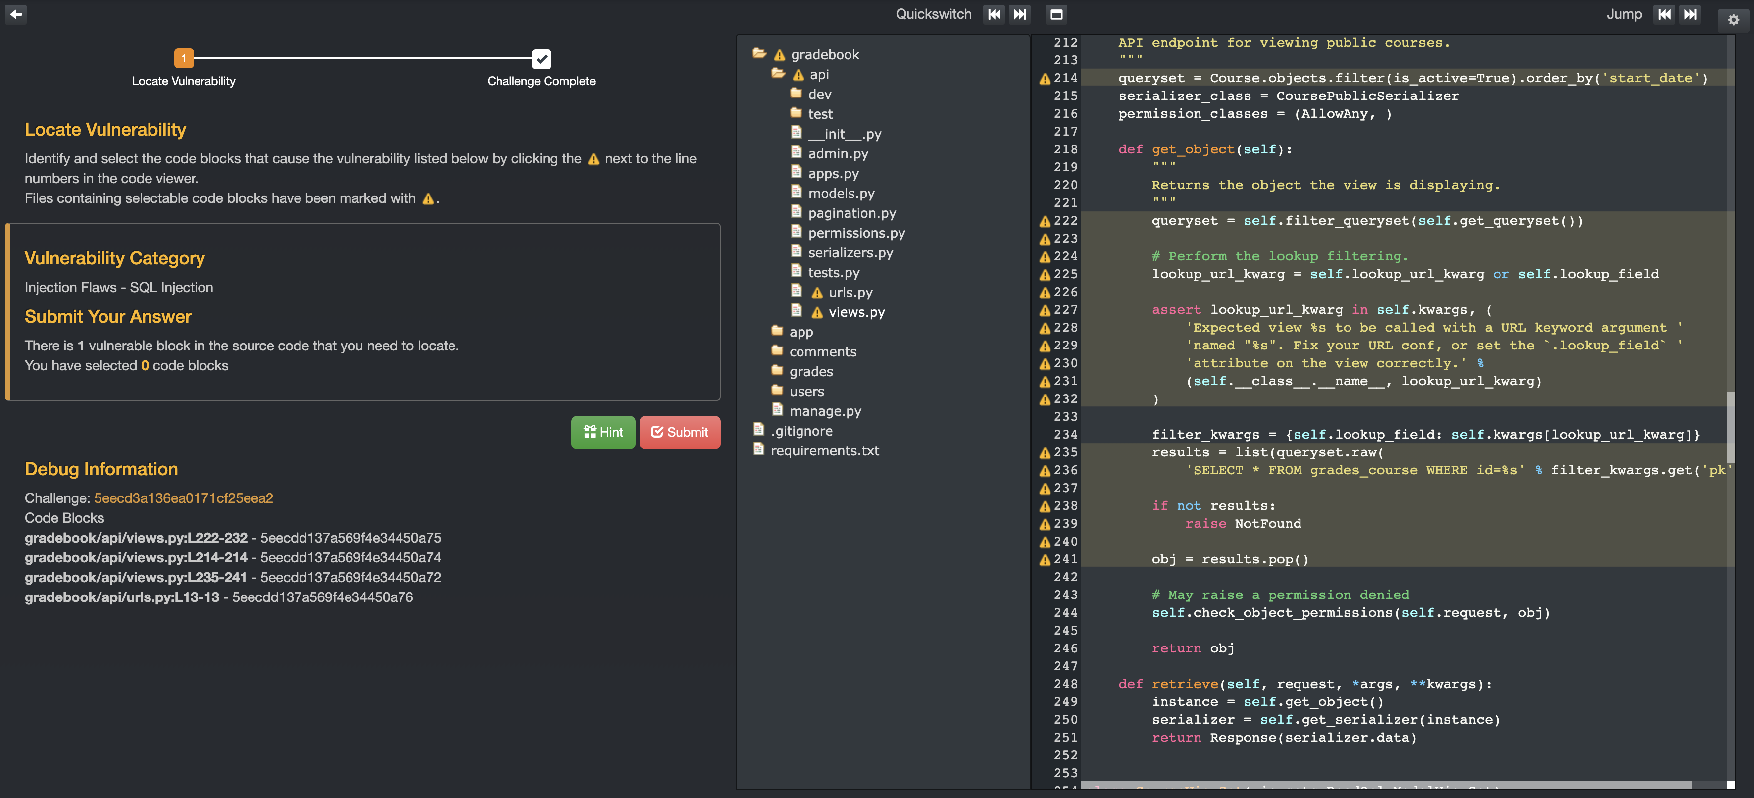
\includegraphics[width=0.95\linewidth]{locate.pdf}}
%\end{subfigure}
%
%\begin{subfigure}[b]{\textwidth}
%\sidebysidecaption{0.05\linewidth}{0.95\linewidth}{
%   \caption{}
%   \label{fig:fix}}{
%   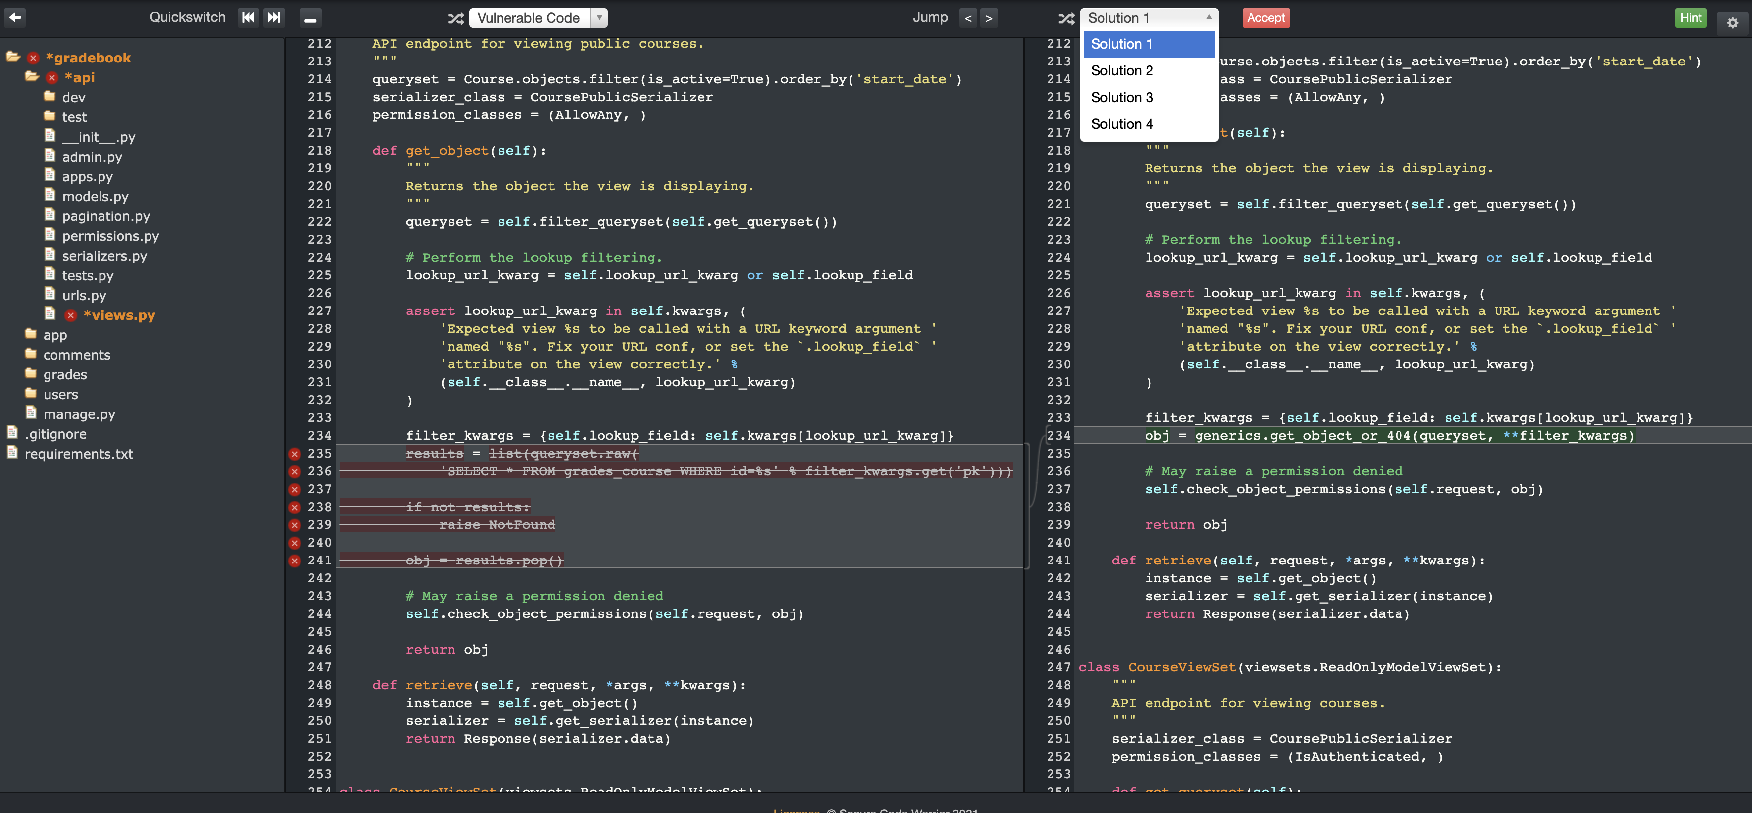
\includegraphics[width=0.95\linewidth]{fix.pdf}}
%\end{subfigure}
%
%\caption[Locate, identify, and fix challenges]{A single vulnerability in a software application can be presented to the developer as three different challenge types. \textit{Identify} exercises (a) mark the vulnerable code fragment and require the developer to select the right category. \textit{Locate} exercises (b) present the vulnerability category and require the developer to select the code fragment containing this vulnerability. \textit{Fix} exercises (c) require the developer to find the secure option among four alternative code bases.}
%\end{figure}

\begin{sidewaysfigure}
  \centering
  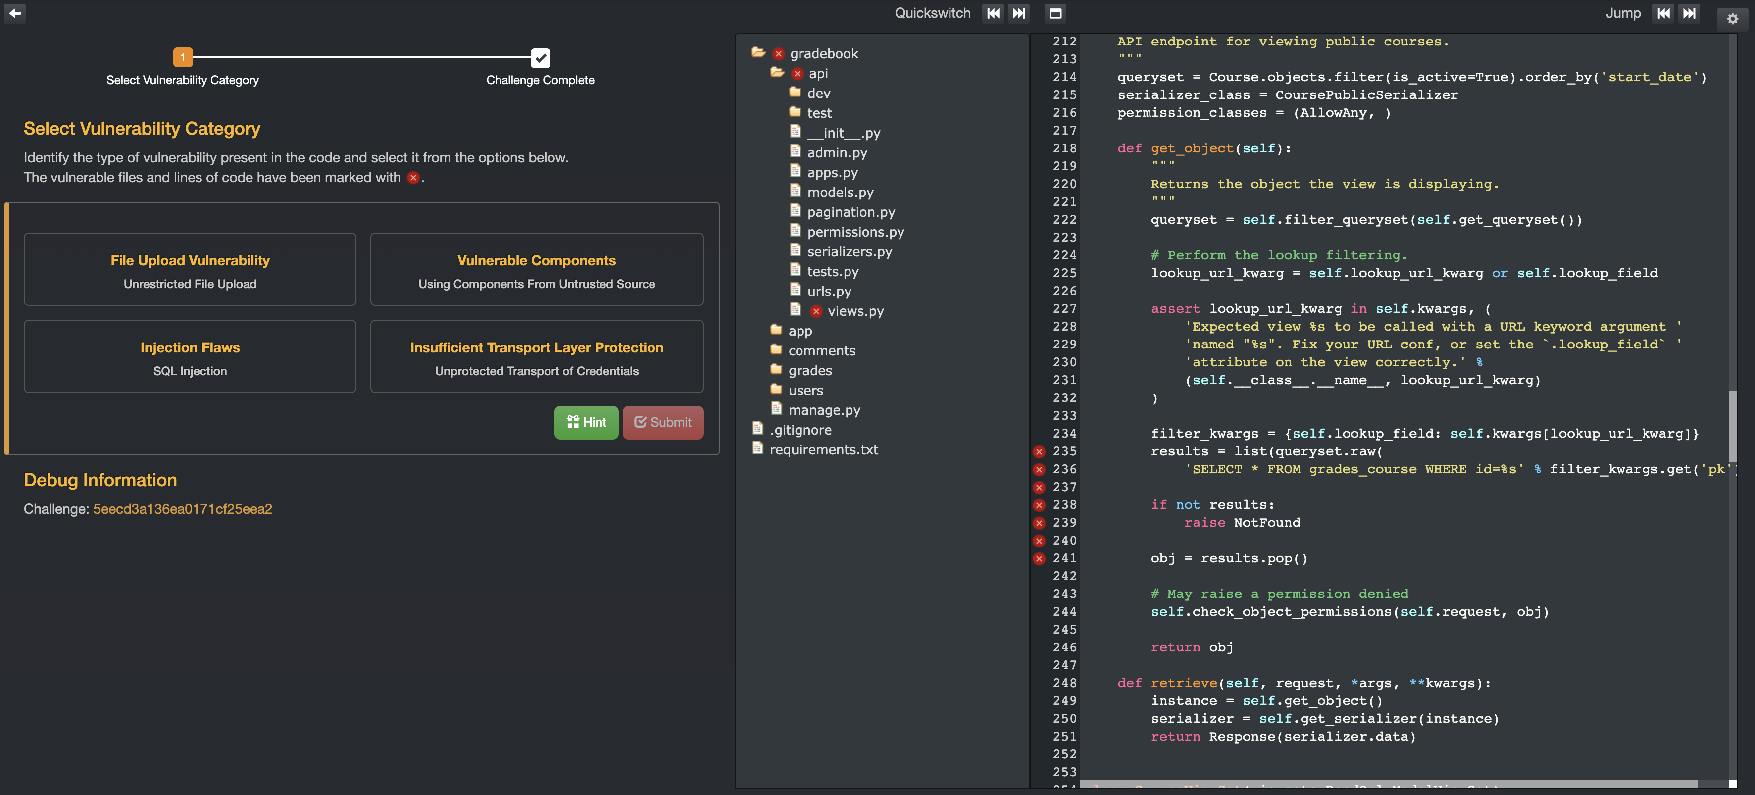
\includegraphics[width=\textwidth]{identify.pdf}
  \caption[Identify challenge]{\Gls{sql} injection in a Python web application presented as an identify exercise, the first of three different challenge types on the \gls{scw} platform.}
  \label{fig:identify} 
\end{sidewaysfigure}

\begin{sidewaysfigure}
  \centering
  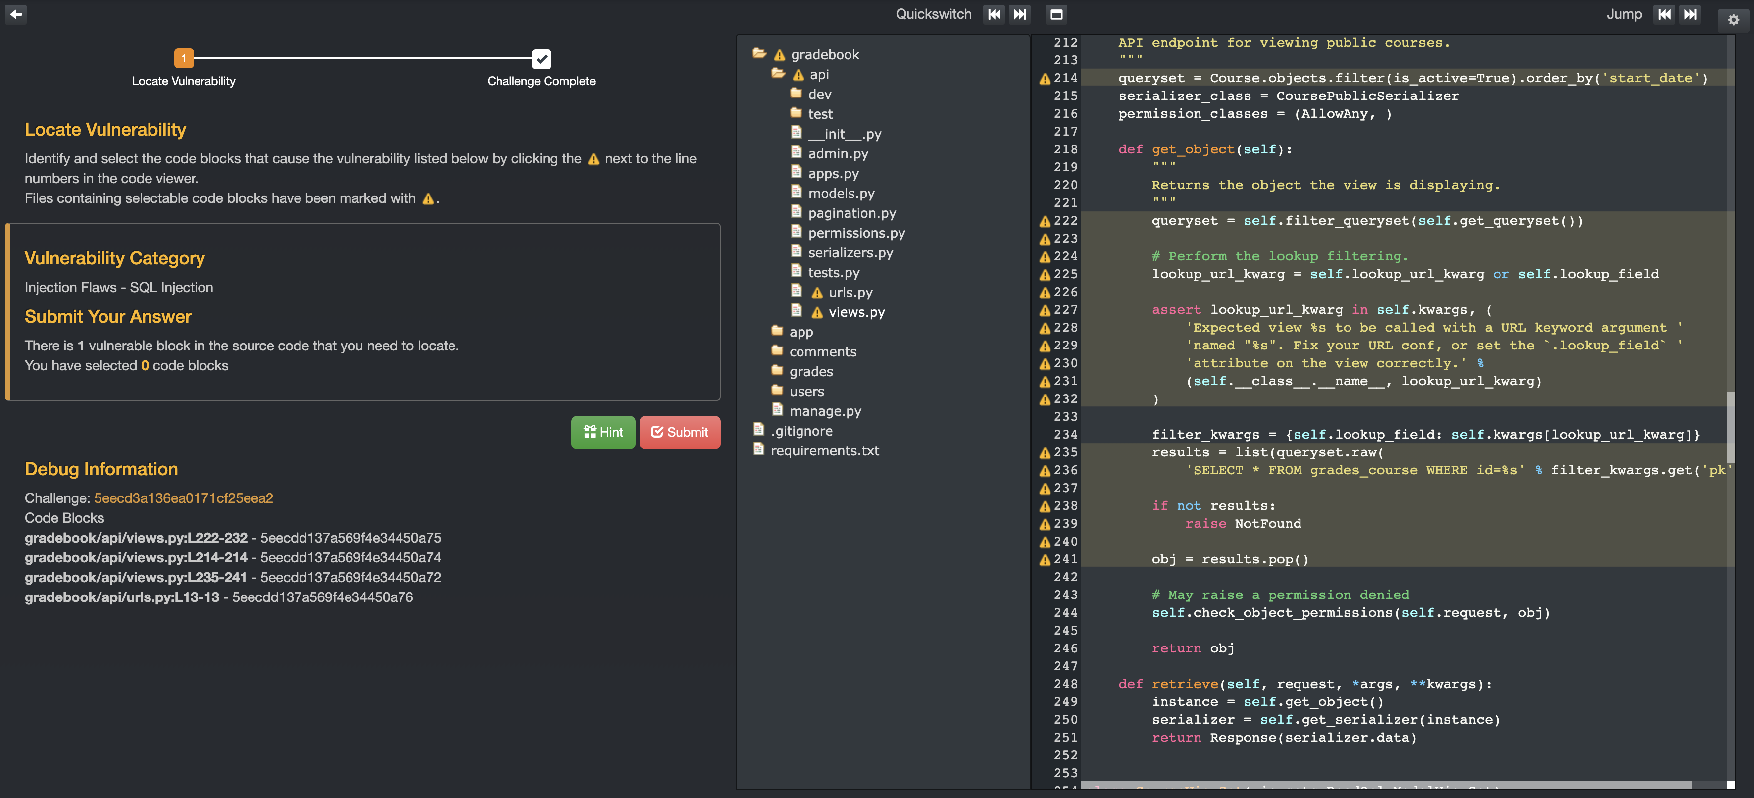
\includegraphics[width=\textwidth]{locate.pdf}
  \caption[Locate challenge]{\Gls{sql} injection in a Python web application presented as a locate exercise, the second of three different challenge types on the \gls{scw} platform.}
  \label{fig:locate} 
\end{sidewaysfigure}

\begin{sidewaysfigure}
  \centering
  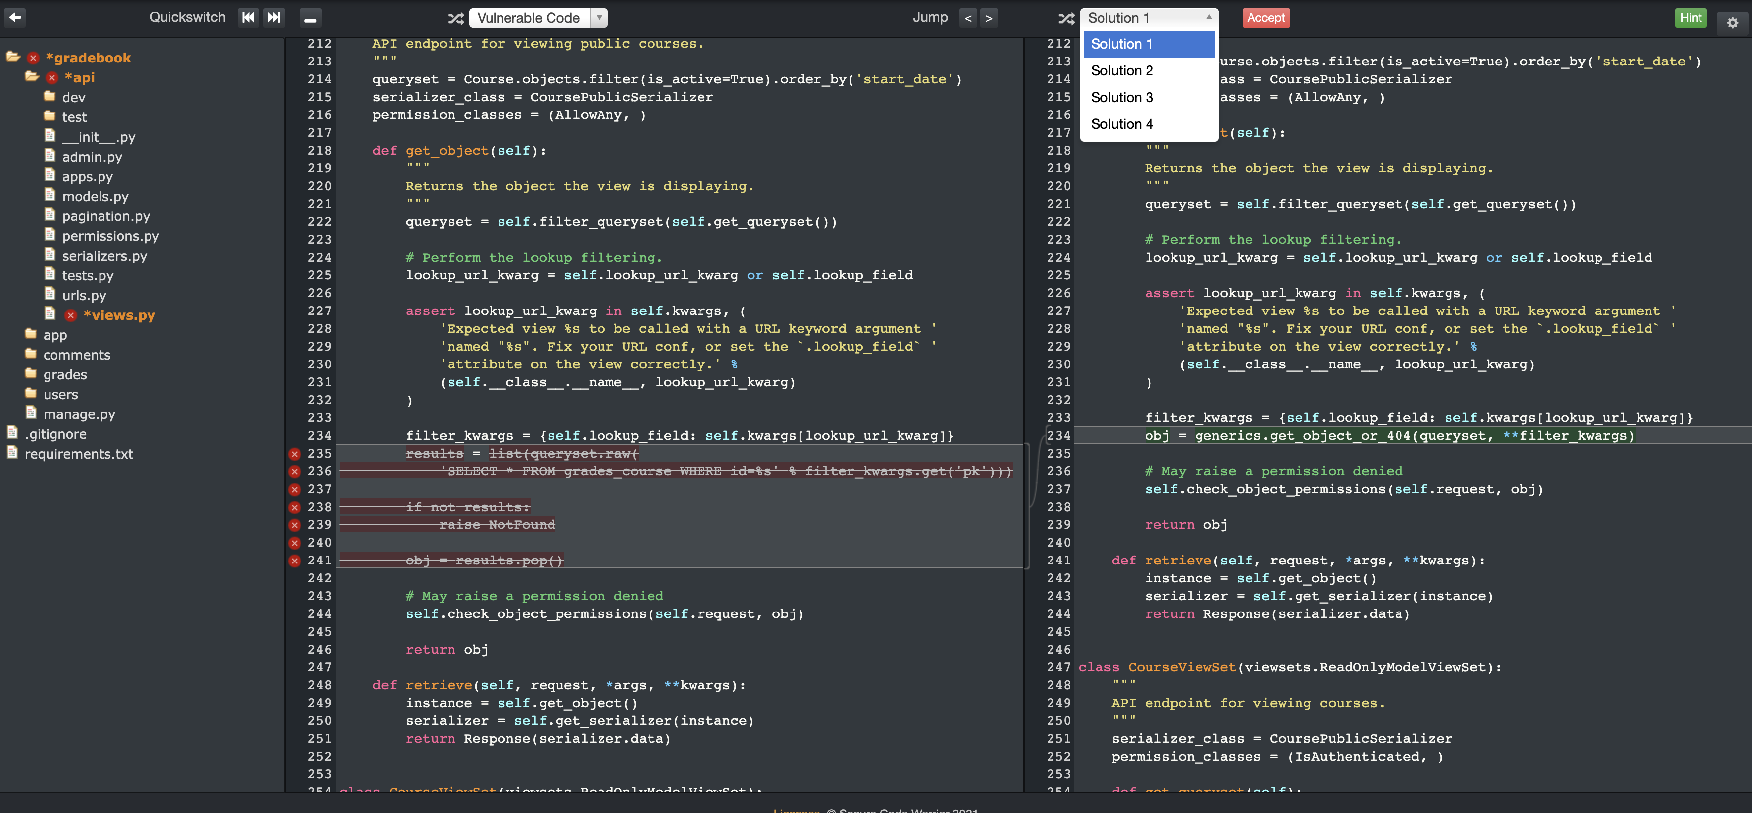
\includegraphics[width=\textwidth]{fix.pdf}
  \caption[Fix challenge]{\Gls{sql} injection in a Python web application presented as a fix exercise, the thrid of three different challenge types on the \gls{scw} platform.}
  \label{fig:fix} 
\end{sidewaysfigure}

Recently new and more interactive challenge types are being developed. 
One such type requires the developer to construct input that successfully exploits the vulnerability present in the application. 

\section{Context}
The challenges are presented to users in different contexts, these are training mode, tournament mode, or assessment mode.

The default context is the training mode.
In this mode the developer is allowed to use as many hints as needed.
They are also allowed an unlimited amount of attempts to find the right answer.
Each hint or failed attempt reduces the amount of points that the developer is awarded.
Appendix~\ref{app:challenges} describes in more detail how the difficulty of a challenge, the amount of hints used, and the number of failed attempts determine how many points are awarded. 
Developers are free to choose which challenges they solve first in training.
A standard course that guides them through the \gls{owasp} Top 10 categories is provided, and many developers complete this course before trying other challenges.

In tournament mode, the scoring method and availability of hints and attempts can be adjusted by the host.
In this mode, all participants are shown exercises about the same vulnerability type and of the same difficulty but in their language of choice.
The tournament is run for a limited time, usually a few hours, in which the contestants can complete the challenges.
In tournament mode, a live leaderboard is visible that can optionally be hidden close to the end for suspense.
Since all participants are shown the same number of exercises having the same difficulty, it often comes down to speed to finish the challenges in time, and accuracy to lose as few points as possible through hints or mistakes.

In assessment mode no hints are available and only one attempt is allowed for each challenge. This mode is used to evaluate the performance of a user.
Customers can select the vulnerability type and difficulty of the challenges making up the assessment.
There are some templates provided as an example that test for knowledge of the \gls{owasp} Top 10.

\section{Course material}
The \gls{scw} training portal provides training in more than 50 languages and frameworks\footnote{\url{https://www.securecodewarrior.com/supported-languages}}, ranging from Cobol to Go, including languages for web, mobile, cloud, and embedded software.
The training content covers 184 different vulnerability types, including those in widely-used lists such as the \gls{owasp} Top 10\footnote{\url{https://owasp.org/www-project-top-ten/}}, \gls{owasp} Top 10 Mobile, \gls{owasp} Top 10 \gls{api} Security and the \gls{cwe} Top 25\footnote{\url{https://cwe.mitre.org/top25}}.
The full list of vulnerabilities can be found on the \gls{scw} website\footnote{\url{https://www.securecodewarrior.com/product/supported-vulnerabilities}}.
This coverage is not homogeneous across all languages.
For each language and framework, each relevant vulnerability type is assigned a priority (high, medium, or low).
This priority depends on the severity and prevalence of the vulnerability type in this particular language and framework combination.

How well a language is covered then depends on the amount of challenges that covers vulnerability types of different priorities. 
The minimum requirement for a language to be considered ready for training is three challenges for each category in the \gls{owasp} Top 10 categories.
A language is considered tournament ready when there are five challenges (two easy, two medium and one high difficulty) for all vulnerability types with high priority, and two challenges (one easy, one medium) for all vulnerability types with medium priority.
There are other requirements still for assessments, specific courses, or the website trial.

For each of the top three frameworks over 450 unique vulnerabilities have been introduced in applications. These frameworks are C\# \gls{mvc} (461 vulnerabilities), Java \gls{ee} \gls{jsp} (475 vulnerabilities), and Java \gls{ee} Spring (495 vulnerabilities). When multiplied by three (for identify, locate, and fix), there are over 1350 challenges for each of these three frameworks.

\section{Use in the paved path methodology}
The \gls{scw} online learning platform is a great educational resource to support the paved path methodology.
The platform is \textit{relevant}, the learning context resembles the developer's work context as they are able to receive training in their office or home office and by looking at actual code. 
The code on the platform is likely to be similar to that of the developer due to the wide variety of programming languages, frameworks, and software types that are supported. 
The exercises teach a developer a secure paved path in their framework of choice. The identify, locate, and fix exercises are all defensive tasks created with the developer in mind.

The platform is also \textit{usable} as there are several features to increase interactivity and engagement, such as the gamified theme, leaderboards, tournaments, achievements, and badges.
A structured journey is present in the form of courses, such as the \gls{owasp} Top 10 courses.
The learning material is presented through multiple choice questions.
In newly released exercise, developers are even be allowed to discover the answer through trial and error instead of picking from a list of options.

% the NEED
There is certainly enough content available to allow for sufficient repetition so that the concepts can be committed to memory, with some frameworks providing as many as 1350 challenges.
However, there is no guidance to find the right balance between repetition and \textit{efficiency}.
The exercises often do not match the learning pace of each individual, leading to boredom or frustration.
This is apparent from the challenge completion rate, as only 45\% of users complete more than 30 challenges, the amount of challenges in an \gls{owasp} top 10 course.

When surveyed, some users indicate this possible mismatch in the learning pace.
More than 700 respondents were asked to describe their experience using the \gls{scw} portal after completing a tournament.
To do this, they were able to choose words from a set of options or write their own.
Many respondents selected words indicating their engagement such as interactive (55\%), engaging (53\%), and fun (48\%).
But some also picked words that could indicate an incorrect learning pace, among which challenging (45\%), repetitive (21\%), long (7\%), and boring (4\%).
Only 22 (3\%) respondents wrote down additional words themselves, some of which indicate mismatches in learning pace. 
Two users wrote down tedious, two users wrote cumbersome, one wrote frustrating, and one even went as far as to describe their experience as gambling.

In conclusion, the \gls{scw} online learning platform is a good educational resource when using a paved path methodology. Its defensive exercises and wide support for different programming languages and frameworks make it \textit{relevant} to the developer's work. The gamification and interactivity keep it \textit{usable} and fun. However, when it comes to the \textit{efficiency} of the training, there is still room for improvement, as currently all users are presented with challenges of the same difficulty regardless of their skill level and learning pace.
User feedback indicates that this leads to boredom or frustration for some of the users. 
\chapter{Intelligent tutoring system}
\label{ch:its-implementation}
\glsreset{its}
%(CONTEXT): background for less specialized readers and establish or recalls the importance of the problem
An important aspect of education in the paved path methodology is its efficiency.
Educational activities should not keep the developer from their responsibilities for longer than necessary.
% (NEED): motivates the audience by stating the difference between the desired and actual situation
% ==>shortcomings and goal from my perspective
The efficiency of training on the \gls{scw} platform is lacking.
Because every individual is presented with the same exercises, they often receive training that is too repetitive or too challenging.
%(The TASK) what did I do?
%=> IRT, ITS
I designed an \gls{its} that recommends exercises to each individual at any point in time to provide them with a more appropriate learning pace.
%When evaluating online learning activities, the focus is often wrongfully on completion and dropout rates~\cite{hadi2016driving}. 
%It is perfectly possible, likely even, that learning took place despite the user not completing the course.
%The goal of the \gls{its} should hence be to maximize the opportunity for learning to take place.
% OBJECT
In this chapter, I present the design of the \gls{its} and discuss the used techniques in its implementation in more detail.
%In this chapter we start with an overview of the design of the \gls{its} in Section~\ref{sec:design}.
%In the rest of the chapter we explain the used techniques in more detail.
%First, the collaborative filtering algorithm is detailed in Section~\ref{sec:collab}.
%Next, the psychometric models are discussed in Section~\ref{sec:calib}.

\summarybox{
I designed an \gls{its} that consists of three algorithmic components, one for exercise selection, and one each for estimation of user ability and exercise difficulty.
Exercise selection is achieved through a \gls{cf} algorithm adapted to learning systems.
In such an algorithm, a target user's preference for an exercise is predicted based on the preferences of like-minded users.
Through the use of the psychometric model of \gls{irt}, estimation of both user ability and exercise difficulty can be done at once.
A sanitized data set of over 9 million solved exercises is used to calibrate these algorithms making up the \gls{its}.
}

% SECTIONS
\section{Design}
\label{sec:design}
The design of the \gls{its} shown in Figure~\ref{fig:its-overview} extends the existing functionality of the training platform.
This existing functionality is depicted in orange on the right side of the figure, while components of the \gls{its} are drawn in blue on the left side.
The \gls{its} consists of two loops, it contains three algorithmic components and three types of data collections.

% high level overview of different components of ITS
\begin{figure}
    \centering
    %\input{03-education/plots/its-flowchart-reverse}
    \includegraphics[page=12]{03-education/figures/tikzfigures.pdf}
  \caption[Design of the ITS]{The \Gls{its} consists of two loops. In the main loop, users are served exercises and their answers are processed, before selecting a new exercise. The user history is then regularly used in a secondary loop to estimate both user abilities and exercise difficulties.}
  \label{fig:its-overview} 
\end{figure}

The algorithmic component in the main loop is that of exercise selection.
Selecting the optimal exercise is done through an adapted \gls{cf} algorithm, as will be explained in more detail in Section~\ref{sec:collab}.
In this technique, a recommendation is derived from historical data of like-minded users.
To evaluate this technique, and hence improve it, we need a measure to decide what a good recommendation is.

A useful challenge is a challenge from which the user has learned something and that keeps the user engaged.
That is, a good recommendation system should increase the \textit{ability} of the user, and their \textit{engagement}.
It is easy to keep track of the engagement of the user.
If they continue to play more challenges, that means they stay engaged.
However, in order to determine if a recommendation leads to increased ability, we need to be able to continuously measure the ability of each user.
Another reason to continuously measure the ability of each user is the temporal aspect to learning.
An exercise that is useful to a user at the beginning of their journey is likely no longer an appropriate recommendation once their ability has sufficiently increased.
Hence ability estimation is needed to both determine \textit{if} a challenge was useful to a user, and \textit{when} a challenge was useful.

A very naive way to achieve an ability estimate is simply looking at the accuracy of each user.
A user answering all of the challenges correctly (100\% accuracy), is likely to have a higher ability level than a user answering half of them correctly (50\% accuracy).
If all users completed the exact same challenges, this could give a reasonably accurate representation of their ability level.
In fact, that is exactly the reasoning behind \gls{ctt}~\cite{ctt}.
In a classic test all examinees are given the same (or equivalent) exercises and their accuracy on the test is an indication of their ability level.

However, on the training platform not all users are completing the exact same challenges and this is not desirable, as that would conflict with the goal of individually tailored recommendations.
When users are completing different challenges, accuracy alone is no longer sufficient.
It is possible for one user to maintain a high accuracy doing simple challenges, while another user's accuracy is lower but they are completing difficult challenges.

This is also true for exercises, the difficulty of an exercise can not be accurately estimated through the accuracy of users completing it.
It is possible for one exercise to have a high accuracy because it is mostly attempted by users of a high ability level, while another is often tried by beginners and hence has a lower accuracy.
It is clear that these two remaining algorithmic components in the \gls{its} are tightly coupled.
Both are implemented through the use of psychometric models from the field of \gls{irt} as explained in Section~\ref{sec:calib}.
The calibration techniques of \gls{irt} use the entire user history and take a while to complete.
This is why they are not performed every iteration of the main loop, but at regular intervals in a secondary loop.

\section{Collaborative filtering}
\label{sec:collab}

In this section, I discuss the first algorithmic component of the \gls{its} as depicted in Figure~\ref{fig:its-overview}, the component of exercise selection.

There are many possible factors that determine which exercise to select.
We can easily imagine some factors that are likely to have a big influence, such as the difficulty of the exercise, the vulnerability type, and the programming language.
Research has also shown that individual learning style has an impact on learning performance~\cite{alshammari2015design,schiaffino2008eteacher,graf2006representative,felder1988learning}.
For other factors, it is more difficult to determine how important they are, or if they matter at all.
Some examples are code quality, code legibility, software type, or even just the coding style of the author of the challenge.
There are also likely other factors that we are not yet aware of.

For this reason, it is desirable to create a recommendation system that uses a black box approach.
With this kind of approach it is not necessary to know which factors determine a good recommendation.
There only need to be enough users and challenges, as well as a way to determine if a challenge was useful to a user.

One frequently used technique for recommendation systems is \gls{cf}.
In \gls{cf}, a target user's affinity for items is used to find other users who are most like-minded.
This group's collective affinity for items is then used to predict the target user's affinity for those items.

These types of algorithms are most easily understood through a visual representation. 
In Figure~\ref{fig:cf}, a simple example of a \gls{cf} algorithm is illustrated.
In this figure, the recorded affinity of users $i$ $(i = 0,\dots,5)$ for movies $j$ $(j = A,\dots,J)$ is depicted in a two dimensional grid.
A green check mark in the grid means that the user enjoyed the movie, a red cross means they did not.
There are also many empty spaces as not all users have watched all movies.
In order to predict the affinity of a target user $i = 0$ for a target movie $j = B$, the \gls{cf} algorithm starts by finding the users who are most like-minded, the users who have the most similar recorded affinity.
For each user, the algorithm determines for how many movies they have the same affinity as the target user.
In Figure~\ref{fig:cf}, the affinity of the target user is marked with an orange background, affinity of other users that is the same as the target user is marked with a green background.
In the example, user $i = 1$ enjoyed movies $j \in \{A,C\}$.
But their affinity for movie $C$ is the only affinity they have in common with the target user.
Users $i \in \{2,3,5\}$ each have the same affinity as the target user for two of the movies. 
In this example, they make up the group of people that are most like-minded to the target user.
To predict if the target user would enjoy the target movie $j = B$, the algorithm now uses this group's affinity for the target movie, marked in a blue background in Figure~\ref{fig:cf}.
Two of the most like-minded users enjoyed the movie and one of them did not.
Since the majority of like-minded users enjoy the target movie, the algorithm predicts the target user might enjoy it as well.

\begin{figure}
    \centering
    %\input{03-education/plots/collaborative-filtering}
    \includegraphics[page=7,width=\textwidth]{03-education/figures/tikzfigures.pdf}
    \caption[Collaborative filtering algorithm]{Visual representation of the steps to determine if the target movie $j=B$ is a good recommendation for the target user $i=0$. 
    The \gls{cf} algorithm first finds all users who have similar preferences for movies as the target user (marked in green). 
    The users who have the most similar preferences are used in a majority vote. 
    In the example users 2, 3, and 5 each had the same preference as the target user for two different movies.
    The majority of these users enjoyed the target movie (marked in blue), so the algorithm concludes that the target is a good recommendation.}
    \label{fig:cf}
\end{figure}

\subsection{Adapted to learning systems}
\label{sec:adapted-cf}
Some adjustments are needed to apply \gls{cf} to a learning system.
In a learning system, a good recommendation is one that allows meaningful learning to take place and at the same time keeps the user engaged.
A good recommendation is hence based on the \textit{utility} of a user for an item, rather than their affinity.
If the users who are most like-minded increased their ability level through playing this challenge, it is likely a good recommendation.

As mentioned before, learning also has a more apparent temporal aspect to it.
An exercise that is useful to a user at the start is no longer an appropriate recommendation once their ability has increased sufficiently.
It could hence be beneficial to keep track of the ability level around which a recommendation can be deemed appropriate.
The \gls{cf} algorithm can then only consider users to be like-minded, if they experienced the same utility as the target user within a certain ability range.
Users who experienced the same utility for an item but at a sufficiently dissimilar ability level will not be considered like-minded users.

Figure~\ref{fig:3d-cf} illustrates how this adaptation could be achieved on the example algorithm from before.
In this figure, the recorded utility that the users $i$ $(i = 0,\dots,5)$ experienced from challenges $j$ $(j = A,\dots,J)$ is depicted in a two dimensional grid for three sufficiently distinct ability levels $\bm\theta$.
A green check mark means that this challenge was useful to the user around that ability level.
A red cross means it was not useful, and the user either did not learn anything, or the challenge caused the user to disengage from the training.
How the utility of a challenge is determined will be explained in Section~\ref{sec:utility}.
To predict the utility of the target challenge $j = B$ to the target user $i = 0$, the adapted \gls{cf} algorithm looks for the most like-minded users, the users who experienced the most similar utility.

However, only if the same utility was experienced around the same ability level does it count towards like-mindedness.
In Figure~\ref{fig:3d-cf}, utility that was experienced by the target user for challenges is marked with an orange background.
Similar utility that was experienced around the same ability level is marked with a green background.
At the lowest ability level, user $i = 2$ experienced the same utility as the target user for four challenges.
User $i = 1$, just like the target user, experienced challenge $j = C$ as useful.
However, the challenge was useful to user $i = 1$ at the lowest ability level, while the target user found this challenge useful when their ability level was sufficiently higher.
Similar utility like this that was experienced around a different ability level is marked with a red background in the figure.
This utility does not count towards like-mindedness.
Using this metric for like-mindedness, we find that users $i \in \{2,3,5\}$ each experienced the same utility around the same ability level as the target user for four different challenges.
They make up the group of users who are most like-minded to the target user.

Beyond this adaptation, the same steps are used to decide the final recommendation.
The majority of like-minded users experienced the target challenge as useful around the targeted ability level, marked with a blue background.
The algorithm concludes that the target challenge is a good recommendation for the target user.

\begin{figure}
    \centering
    %\input{03-education/plots/3d-collaborative-filtering}
    \includegraphics[width=\textwidth,page=3]{03-education/figures/tikzfigures.pdf}
    \caption[Adapted collaborative filtering algorithm]{Visual representation of the steps to determine if the target challenge $j=B$ is a good recommendation for the target user $i=0$. 
    The collaborative filtering algorithm first finds all users who experienced similar utility from challenges as the target user around the same ability level $\bm\theta$ (marked in green). 
    Similar utility at a different ability level is disregarded (marked in red).
    The users who experienced the most similar utility are used in a majority vote. 
    In the example, users 2, 3, and 5 each experienced the same utility as the target user for four different challenges.
    The majority of these users experienced the target challenge as useful (marked in blue), so the algorithm concludes that the target is a good recommendation.}
    \label{fig:3d-cf}
\end{figure}

\subsection{Types of collaborative filtering}
In the examples until now, the affinity (or utility) of a user for an item was considered binary, the user either liked it, or they did not.
In reality, often a more complex scale is used.
For example, Netflix movie recommendations use a rating scale between 1 and 5.
In this context, the affinity of a user $u$ for an item $i$ is often called the rating $r_{ui}$.
The goal of a \gls{cf} algorithm is then to make a prediction for this rating $\hat{r}_{ui}$.
\Gls{cf} algorithms can be split into two broad categories, memory-based and model-based algorithms, based on how they set out to achieve this goal~\cite{li2021novel,sharma2017collaborative,yu2004probabilistic,breese2013empirical,su2009survey}.

\subsubsection{Memory-based}
Memory-based \gls{cf} algorithms directly use observed ratings to compute predictions.
Generally, these algorithms mark a subset of users as neighbours to the target user by calculating the similarity between users~\cite{li2021novel,Hug2020}.
They then use the neighbour's ratings to predict the rating of the target user~\cite{su2009survey,Hug2020,Koren2010,Ricci2010}.

Memory-based \gls{cf} algorithms are frequently used in recommender systems and even commercial systems such as the Amazon webstore~\cite{sharma2017collaborative,yu2004probabilistic}.
The main advantages of memory-based collaborative filtering algorithms are that they are easy to implement, and that new data can be added easily and incrementally.
Their biggest shortcoming is a decreased performance for sparse data, when it is difficult to find sufficient neighbours.
They also can not make recommendations for new users or items as there is no data to do similarity computations with.
In the \gls{its} however, we already need sufficient data to compute the difficulty and ability estimates.
In a learning system, the need for an initial calibration phase can not be avoided, so this shortcoming does not impact the design of the \gls{its}.

Five different memory-based \gls{cf} algorithms are considered in this work. 
They will be described in more detail in the experiments in Section~\ref{sec:eval-cf}.
Four of these algorithms are \gls{knn} algorithms, they first determine the k nearest neighbours and then use the ratings of these neighbours to compute a prediction.
Because these algorithms use an explicit definition of similarity between users, they can be easily adapted to learning systems by changing this definition to take into account the ability of the users.
The remaining memory-based algorithm uses the ratings of all users to make a prediction, adapting it to learning systems will be harder, but can still be achieved by processing the data, as will be explained in the description of the experiments.

\subsubsection{Model-based}
Model-based \gls{cf} algorithms use statistical and machine learning methods to construct a model, and use this model to make predictions~\cite{sharma2017collaborative, li2021novel,sarwar2002recommender,heckerman2000dependency}.
These models often use techniques to reduce the dimensions of the matrix of user-item ratings.
This reduces the scalability and sparsity problems that are experienced by memory-based algorithms~\cite{sarwar2002recommender,moreno2016web}.
Model-based algorithms are often more accurate, but the construction of the model is often slow and expensive, and they have to be re-built regularly, every time new data is being added incrementally.

Algorithms using clustering techniques are simple examples of model-based algorithms~\cite{su2009survey,breese2013empirical,sarwar2002recommender,o1999clustering}.
Users or items are assigned to one or more clusters so that the matrix of user-item ratings becomes a smaller, denser matrix of clusters.
It is then possible to use statistics from these clusters to make predictions, for example, by taking the average rating of a cluster.
In the experiments of this work, one clustering algorithm is evaluated.

Thanks to their accuracy and scalability, model-based algorithms based on matrix factorization have gained a lot in popularity~\cite{Ricci2010}.
These algorithms use the technique of \gls{svd} to make a low rank approximation of the original ratings matrix~\cite{george2005scalable, Ricci2010, Hug2020}.
\Gls{svd} is a well-established technique in linear algebra and machine learning to identify latent semantic factors.
Applying it in the \gls{cf} domain raises a few difficulties due to the sparsity of the rating matrix, which increases the risk of overfitting.

In the experiments of this work, I evaluated \gls{pmf}~\cite{mnih2008probabilistic}, \gls{nnmf}~\cite{wang2012nonnegative,hoyer2004non}, \gls{svd}~\cite{sarwar2000application,polat2005svd,Ricci2010}, and \gls{svd}++~\cite{koren2008factorization,Ricci2010}.
All of these algorithms are explained in more detail in Section~\ref{sec:eval-cf}.

\subsection{Alternative approaches}
\label{sec:cf-alternatives}
Many existing alternatives either do not take into account the ability level of the users to make recommendations, or they only take into account the ability level~\cite{chen2005personalized}.

\subsubsection{Adaptive learning systems}
Many computerized learning systems already exist, both in commercial offerings and in research literature.
Older systems do not consider individual learners needs, but make decisions based on pre-planned instructions for the field of study.
As a result, these systems do not provide individual attention to students as a natural (human) teacher would~\cite{mahdi2016intelligent}.
This inspired the rise of more advanced learning systems that consider both the field and the learner to provide flexibility in the presentation of the educational material.
Some such systems have been built to teach computer science concepts, such as debugging~\cite{carter2013tutoring}, cryptographic algorithms~\cite{abuel2018intelligent,mahdi2016intelligent}, programming in C++~\cite{abu2009evaluating}, or \gls{sql}~\cite{mitrovic2003intelligent}.

These systems have varying degrees of intelligence and adaptiveness.
In commercial offerings, such as Pluralsight Iris\footnote{\url{https://www.pluralsight.com/product/iris}}, adaptive learning often refers to an initial calibration phase to determine the initial ability level of a user.
In other systems, students are allowed to advance to more difficult levels when a sufficiently high accuracy is achieved on exercises in the current level~\cite{abu2009evaluating,mahdi2016intelligent}.
Even more advanced systems provide adaptive feedback to the users, based on which mistakes have been made in the exercises~\cite{carter2013tutoring,abuel2018intelligent}.
Finally, the most advanced systems are able to adapt the difficulty of the exercises more dynamically.
Duolingo for example, adapts the difficulty of the of last few exercises in a lesson based on the performance of the student on the previous exercises\footnote{\url{https://blog.duolingo.com/}}.

All of these system focus on offering exercises of the appropriate difficulty level, and some also take into account classifications of learning styles~\cite{alshammari2015design,felder1988learning}.
The goal of the \gls{its}, however, is to also pay attention to other potential factors such as the coding style, presentation form, application type, and so on.
The discussed systems could potentially be adapted to take into account several of these factors.

\subsubsection{Serious games}
Several serious games exist to for topics related to cybersecurity and social engineering.
They usually focus on increasing the awareness of software users of different ages and are not used to train software developers~\cite{giannakas2015cyberaware,jin2018evaluation,beckers2016serious,yasin2018design}.

Research in this field mostly focuses on the effect of gamification, and usually adds game elements to static learning content.
They usually do not adapt to the users beyond opening up new content after the completion of preceding exercises.
While gamification leads to increased engagement, this is not the focus of my research as I believe the \gls{scw} platform already has some decent gamification features.

\subsubsection{Content-based recommendation systems}
Another type of recommendation system that is related to \gls{cf} algorithms, is content-based recommenders.
These systems analyze item descriptions to identify items that are of particular interest to a user~\cite{pazzani2007content}.
To do this, they represent both items and users as a vector of characteristics, similar to vectors in the latent space used by model-based \gls{cf} algorithms.
However, in contrast with these \gls{cf} algorithms, the vectors are not computed in a latent space by the algorithm.

Item characteristics are often already available in the system, or they can be detected through natural language processing.
They are often easier to interpret than the dimensions of the latent space in model-based algorithms.
On the \gls{scw} platform, the framework, language, vulnerability type, and author are examples of characteristics that are readily available.

In order to make a recommendation for a user, items are selected that have similar characteristics to previously liked items by this user.
Several algorithms can be used to achieve this, among which nearest neighbour methods and decision trees~\cite{pazzani2007content}.
In contrast with item-based collaborative filtering, these algorithms compute the similarity between items based on the characteristics of the items themselves.
While in \gls{cf} algorithm the similarity between items is based on the similarity of ratings these items receive by users.
This is likely not a good approach for learning systems, where diverse content should be recommended, covering, for example, multiple vulnerability types.

\subsubsection{Knowledge-based recommendation systems}
Systems that make use of the organisation of learning material are called knowledge-based, or semantics-based recommendation systems.
They create a structured knowledge graph or ontology to organise the learning material.

Existing ontologies in software security attempt to organize different security concepts in a broader knowledge graph of computer science.
For example, they classify \gls{sql} injection as a type of injection attack, \gls{sql} security as a type of data integrity, and a \gls{dos} attack is linked the availability of the product~\cite{kang2013security, jia2018practical}.
While this information can be useful to a developer learning about different security concepts, it can not be used to organise the learning material on the \gls{scw} training platform.

Many vulnerability types require a broad knowledge of varying aspects of software development, such as the operating system, communication protocols, language and framework specifics, software architecture, and more.
On the \gls{scw} platform, however, we assume the users have sufficient knowledge of these domains, and require education in software security only.
With this assumption, I do not see a need to create a knowledge graph for software vulnerabilities.
It is my belief that most vulnerabilities are unrelated to each other, in the sense that it is possible to understand and master each of them without the need to learn about the other.
Current education efforts often focus on the \gls{owasp} top 10, in which vulnerabilities are ranked mostly based on their prevalence in practice.
This is strong evidence for the fact that the order they are being taught to developers is not of big importance.

\subsubsection{Computerized Adaptive Tests}
\Glspl{cat} are computer-based tests that adapt to the ability of the examinee. 
They continuously estimate the ability level and serve the next test item based on the current estimate.
While there are techniques from \glspl{cat} that are useful to us, as will be explained in Section~\ref{sec:calib}, the item selection is not appropriate for use in the \gls{its}.

This is because the goal of a test is to estimate the ability of an examinee. \Glspl{cat} are able to maintain a higher precision of ability estimation while being about 50\% shorter compared to \glspl{fit}~\cite{weiss1984application}.
To estimate the examinee's ability in such an efficient way, \glspl{cat} select the next item in a test based on which one provides the most information about the examinee. 
These are the items for which the probability of a correct answer is around 50\%~\cite{magis2017computerized, ling2017computerized}.

This goal is of course different from that of the \gls{its} which is to motivate and engage the users. 
In fact, the opposite is even true, tests are inherently not very motivating.
Certainly that is the case for \glspl{cat}, where the examinee is only expected to correctly answer half of the test questions.
Research has shown that engagement can be improved, and anxiety reduced, by choosing items for which the probability of a correct answer is higher (e.g. 70\%)~\cite{ling2017computerized}. 
Still, the item selection algorithm in \glspl{cat} only takes into account the difficulty of the items. 
As discussed before, we want the \gls{its} to possibly take into account other aspects of the exercises, such as coding style, author, or application type.
\section{Difficulty estimation and ability estimation}
\label{sec:calib}
% These two are not always independent:
% Getting difficult challenges correct should have more impact than getting easy challenges correct
% Skilled users answering an exercise correct should have a different impact than unskilled users answering an exercise incorrect

%Difficulty is based on the amount of options this challenge has in the identify stage. Completely irrelevant for the other stages. And not related at all to the code quality, vulnerability type, code complexity etc
%Mention exact algorithm here!

%A score is rewarded to players after completion
%Based on performance and difficulty of the challenge
%the high score also does not accurately represent skill level

% Ability level is needed for two tasks in the system:
% 1. We need accurate absolute ability estimation for temporal aspect of a recommendation
% 2. and fast relative ability estimation for deciding if a challenge is useful or not
In the previous section, I discussed the component of exercise selection, the first algorithmic component of the \gls{its} as shown in Figure~\ref{fig:its-overview}.
This algorithmic component is implemented through the use of a \gls{cf} algorithm.
In order to use this algorithm effectively in a learning system, we need an accurate ability measure.
This ability measure is necessary to both determine \textit{if} a challenge was useful, and \textit{when} a challenge was useful.
In this section, I discuss ability estimation, together with difficulty estimation, the two remaining algorithmic components of the \gls{its}.
I explain how both can be implemented simultaneously by using \gls{irt}, a technique borrowed from the field of psychometrics.
This field of study focuses on the objective measurement of skills, knowledge, and abilities, often with the goal to create better computerized tests.

The goal of a test is to estimate the ability of an examinee.
With \glspl{cat}, this can be done with higher precision while using less exercises than classic \glspl{fit}.
To achieve this, \glspl{cat} continuously adapt the exercises to the estimated ability level of the examinee.
An overview of the steps taken by a \gls{cat} is shown in Algorithm \ref{al:test}. 

\begin{algorithm}[H]
\SetAlgoLined
\SetKwInOut{Input}{\textcolor{scw-red}{input}}
\SetKwInOut{Output}{output}
\Input{calibrated item bank $I$}
\Output{ability level $\bm{\theta}$}
Set $\bm{\theta}$ to entry level\;
\While{termination criterion not met}{
  Select optimal item $i$ from $I$ based on $\bm{\theta}$\;
  Present $i$ to examinee\;
  Update $\bm{\theta}$ based on all prior answers\;
 }
\caption{\label{al:test}A computerized adaptive test}
\end{algorithm}

Some key components are needed to create such a test: calibrated test items, a termination criterion, a starting point or entry level, an item selection algorithm, and an ability estimation algorithm.
We can easily see parallels between a \gls{cat} and the \gls{its}. 
First, test items in a \gls{cat} need to be calibrated, similarly to the exercises in the \gls{its}. 
Secondly, it is necessary in both systems to continuously estimate the ability of the users. 
Finally, there is also a selection algorithm that determines which item the user is shown next. 
However, the item selection algorithm in a \gls{cat} is designed with a different goal in mind, as discussed in Section~\ref{sec:cf-alternatives}. 

\Glspl{cat} frequently use the psychometric model \gls{irt}.
This model not only allows calibration of both users and items, but because they are placed on the same scale, the results can easily be used for item selection as well.
Although it will not be used for exercise selection in the \gls{its}, the model is certainly useful for accurately estimating exercise difficulty and user ability. 

\subsection{Item response theory}
\label{sec:irt-intro}
\Gls{irt} is a model for measuring psychological \textit{latent traits}, i.e. unobservable characteristics such as ability or competence level. 
The model estimates these latent traits by means of \textit{manifest} (observable) variables and statistical psychometric models.
This is done based on the mathematical relationship between the latent traits and the manifest variables. 
A user with a higher ability level (latent trait) is more likely to answer more questions, and more difficult questions, correctly (manifest variables). 
This relationship can be written down as a mathematical function, called the \gls{irf}. It describes the possibility of observing each possible answer as a function of person ability levels and exercise parameters.

\begin{equation}
    \label{eq:irf}
    P_{jk}(\bm{\theta}_i,\bm{p}_j) = Pr(X_{ij} = k | \bm{\theta}_i,\bm{p}_j) = f(k,\bm{\theta}_i,\bm{p}_j)
\end{equation}

In Equation \ref{eq:irf} the ability level of a person $i$ $(i = 1,\dots,I)$ is represented by a multivariate vector of latent traits $\bm{\theta}_i$. $\bm{p}_j$ is the set of parameters of exercise $j$ $(j = 1,\dots,J)$. $X_{ij}$ is the answer of person $i$ for exercise $j$, with $k$ representing one possible answer. 
For dichotomously scored exercises (e.g. true/false) $k \in \{0,1\}$, for polytomously scored exercises (e.g. multiple choice) $k \in \{0,\dots,K_j\}$. 
There are many mathematical functions that can be used to describe the \gls{irf}, each resulting in a different \gls{irt} model.
The most common, and the one used in the \gls{its}, is called the Rasch model, and will be explained in the next Section.

The Rasch model is a dichotomous model.
It is necessary to use a dichotomous model in the \gls{its} because some important data is missing to use polytomous models effectively.
Polytomous models are most effective when the number of possible options for the multiple choice question is limited to three or four. 
The incorrect options need to be deliberate and able to mislead a person with a lower ability level. 

On the \gls{scw} training platform, this is not the case as will be explained in Section~\ref{sec:data}.
Because of this lack of useful polytomous information, I decided to use the dichotomous Rasch model.
For dichotomous models, there are only two outcomes, $k \in \{0,1\}$, representing correct and incorrect.
That means the \gls{irf} in Equation \ref{eq:irf} can be reduced to

\begin{subequations}
\label{eq:irf-dicho}
\begin{align}
        P_{j1}(\bm{\theta}_i,\bm{p}_j) = Pr(X_{ij} = 1 | \bm{\theta}_i,\bm{p}_j) &= P_{j}(\bm{\theta}_i,\bm{p}_j) ,         \label{eq:irf-dicho1} \\
        P_{j0}(\bm{\theta}_i,\bm{p}_j) = Pr(X_{ij} = 0 | \bm{\theta}_i,\bm{p}_j)
        &= 1 - P_{j}(\bm{\theta}_i,\bm{p}_j)
        = Q_{j}(\bm{\theta}_i,\bm{p}_j) ,         \label{eq:irf-dicho2}
\end{align}
\end{subequations}

such that $P_{j}$ represents the probability of a correct response for exercise $j$, and $Q_j$ the probability of an incorrect response.

\subsection{Rasch model}
\label{sec:rasch}
Several mathematical functions can be used to characterize the \glspl{irf} in Equations \ref{eq:irf-dicho1} and \ref{eq:irf-dicho2}.
The most commonly used are logistic distribution functions, resulting in the so-called Rasch model~\cite{rasch1960probabilistic}.

%\todo[inline]{Add advantages of Rash model here or is this out of scope of the work?}
%Rasch modeling allows for generalizability across samples and items, takes into account that response options may not be psychologically equally spaced, allows for testing of unidimensionality, produces an ordered set of items, and identifies poorly functioning items as well as unexpected responses. Each of these characteristics becomes a potential advantage to be exploited.

%Rasch modeling is new to the field of counseling psychology, and only time will determine whether the advantages are sufficient to warrant use. However, several of the advantages appear promising. For example, the ability to identify unexpected results has research and clinical applications. In classical test models, outliers are identified by extreme scores, but we take scores in the middle ranges to be acceptable, as long as the instrument has generally been shown to be reliable. Rasch modeling would identify a research participant who had responded randomly to the instrument (therefore scoring near the mean) or idiosyncratically to a few items. Similarly, clinicians using scales designed on the basis of Rasch modeling could identify clients who responded unexpectedly (and without resort to separate scales, such as is the case with the Minnesota Multiphasic Personality Inventory).

In its simplest form the Rasch model takes only one parameter $\bm{p}_j = b_j$ representing the difficulty of the exercise. 
The \gls{irf} using a one-parameter logistic distribution function is shown in Equation~\ref{eq:1pl}.

\begin{equation}
    \label{eq:1pl}
    P_{j}(\bm{\theta}_i,\bm{p}_j) =
    Pr(X_{ij} = 1 | \bm{\theta}_i,b_j) =
    \frac{\exp(\theta_i - b_j)}{1 + \exp(\theta_i - b_j)}
\end{equation}

The resulting model is called the \gls{1pl}. 
In Figure~\ref{fig:1pl} the \gls{irf} of the \gls{1pl} model is plotted for three exercises with various values for the difficulty parameter.
In this model, for a fixed ability level $\bm\theta$, the probability of a correct answer $P_j$ is lower for exercises with a larger difficulty $b_j$.
The probability takes the value of 0.5 when the ability level of the user exactly matches the difficulty of the item.
This is a result of placing the user abilities and the item difficulties on the same scale.

\begin{figure}
    \centering
    %\input{03-education/plots/1pl}
    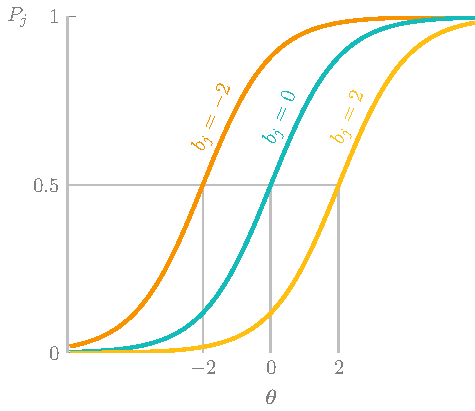
\includegraphics[page=1]{03-education/figures/tikzfigures.pdf}
    \caption[Item response functions of the 1PL model]{Three \glspl{irf} in the \gls{1pl} model, with different difficulty parameters $b_j$. The difficulty parameter represents the difficulty of the exercise. 
    For a fixed ability level, e.g. $\bm\theta = 0$, a higher difficulty means a lower probability $P_j$ of getting a correct answer.
    The probability of a correct answer is 50\% when $b_j = \bm\theta$.}
    \label{fig:1pl}
\end{figure}

There are more characteristics to an exercise than its difficulty. 
One characteristic that is useful to help estimate the ability of users is the discriminative ability of the exercise.
This characteristic represents how good an exercise is at differentiating between users of varying ability levels.
An extension to the \gls{1pl} model exists that includes this parameter, resulting in the \gls{2pl}. 
This second parameter $a_j$ of an item is a multiplicative parameter, as shown in the \gls{irf} in Equation~\ref{eq:2pl}.

\begin{equation}
    \label{eq:2pl}
    P_{j}(\bm{\theta}_i,\bm{p}_j) =
    Pr(X_{ij} = 1 | \bm{\theta}_i,a_j,b_j) =
    \frac{\exp\big[a_j(\theta_i - b_j)\big]}{1 + \exp\big[a_j(\theta_i - b_j)\big]}
\end{equation}

In Figure~\ref{fig:2pl} the \glspl{irf} are plotted for three exercises with the same difficulty $b_j = 0$ but various discriminative abilities. 
For all three \glspl{irf} the probability of a correct answer is still 0.5 for users with an ability level equal to the exercise difficulty.
However, the second parameter influences the steepness of the curve.
For larger discrimination parameters such as $a_3 = 4$, a smaller increase in ability $\bm\theta$ around the exercise difficulty level $b_j = 0$ leads to a more notable increase in probability of a correct answer $P_j$.
Such an exercise discriminates better between low and high ability users.
On the other hand, exercises with lower discrimination values, like $a_1 = 0.25$ result in flatter \glspl{irf} and do not allow as easily for such discrimination.

\begin{figure}
    \centering
    %\input{03-education/plots/2pl}
    \includegraphics[page=2]{03-education/figures/tikzfigures.pdf}
    \caption[Item response functions of the 2PL model]{Three \glspl{irf} in the \gls{2pl} model, with equal difficulty parameter $b_j$ but different discrimination parameters $a_j$. The discrimination parameter represents how well an exercise can differentiate between users of different ability levels $\bm\theta$. A higher value means a steeper increase in probability of a correct answer $P_j$ around the difficulty level $\bm\theta = b_j$.}
    \label{fig:2pl}
\end{figure}

%Figure~\ref{fig:its-architecture} shows the completed architecture of the \gls{its}, obtained by replacing the algorithmic components with the techniques explained in this section.
%
%\begin{figure}
%    \centering
%    \input{03-education/plots/its-filled}
%  \caption{todo}
%  \label{fig:its-architecture} 
%\end{figure}

\subsubsection{Model calibration}
Both the \gls{1pl} and \gls{2pl} models hold parameters of two types: item parameters $\bm{p}_j$ and person parameters $\bm{\theta}_i$. 
With enough data, both sets of parameters can be accurately estimated.
First, the item parameters are estimated independently of the ability levels, this is called the \textit{model calibration}. 
Next, the ability levels are estimated while keeping the item parameters fixed.

\Gls{irt} offers several model calibration techniques, mostly designed for item banks with several dozens of items.
The larger size of the item bank of \gls{scw} will cause longer execution times and more difficult convergence to stable estimates.
I solve this problem by splitting the item bank to several smaller item banks, for example one for each framework on the platform.
The resulting consequences are discussed in Chapter~\ref{ch:its-experiments}.

The calibration of the model consists of tuning the model parameters to maximize the likelihood of the observed data.
More formally, model calibration is maximizing the likelihood of the model $L(\bm\theta,\bm{p})$ with respect to all item parameters $\bm{p} = (\bm{p}_1,\dots,\bm{p}_J)$.
Because this likelihood is also dependent on all person parameters $\bm\theta = (\theta_1,\dots,\theta_I)$, direct maximization is not possible.
There are several possible techniques that can be used to overcome this.
The most well-known are \gls{jml}, \gls{cml}, and \gls{mml}~\cite{magis2017computerized}.

The \gls{jml} algorithm iteratively maximizes the full likelihood with respect to both person and item parameters until convergence is reached.

\Gls{cml} relies on properties specific to the Rasch model to replace unknown ability levels with known sufficient statistics which then allows for the estimation of the item parameters without requiring the estimation of the person parameters.

\Gls{mml} is formulated under the assumption that the ability is a random parameter.
In contrast to the \gls{cml}, it can be used for other \gls{irt} models besides the Rasch model~\cite{bartolucci2010point}.
It does not replace the person parameters by sufficient statistics, but aims to integrate out the person parameters from the maximization process~\cite{bartolucci2010point,magis2017computerized}.
A prior distribution for the ability parameters $f(\bm{\theta})$ is used to compute the marginal likelihood (or the expectation) of a response pattern as shown in Equation~\ref{eq:integrate-out}.

\begin{equation}
    \label{eq:integrate-out}
    P_{j}(\bm{p}_j) = \int_{\mathbb{R}} P_{j}(\bm{\theta}_i,\bm{p}_j) f(\bm{\theta}_i) d\bm{\theta}_i
\end{equation}

The prior distributions are often chosen as normal distributions.
The item parameters can then be estimated by maximizing the full likelihood, calculated as the product of all marginal pattern likelihoods.
Computing these marginal response pattern distributions was conceptually complex until efficient \gls{em} algorithms were implemented~\cite{magis2017computerized}.

In this work, I used the \gls{mml} approach as it has many advantages, such as its applicability to many types of \gls{irt} models, its ability to compare the fit of different models, and its ability to handle perfect response patterns (all correct or all incorrect answers).

\subsubsection{Ability estimation}
Once the item parameters are calibrated, they are set as fixed.
Estimating the person parameters is done through maximizing the \textit{likelihood function} shown in Equation~\ref{eq:wle1}, with respect to $\theta$. 

\begin{equation}
    \label{eq:wle1}
    L(\theta) = \prod_{j=1}^{J} \prod_{k=0}^{K_j} P_{jk}(\theta, \bm{p}_j)^{Y_{jk}}
\end{equation}

In this equation, $Y_{jk}$ equals one if the response category $k$ was chosen for item $j$ and zero otherwise.

Note that since the item parameters $\bm{p}_j$ are already calibrated and now set as fixed, the function only depends on the person parameters $\theta$.
Maximizing this function is equivalent to maximizing its logarithm, the so-called \textit{log-likelihood function}, as shown in Equation~\ref{eq:wle2}.

\begin{equation}
    \label{eq:wle2}
    l(\theta) = \sum_{j=1}^{J} \sum_{k=0}^{K_j} Y_{jk}\log P_{jk}(\theta, \bm{p}_j)
\end{equation}

For dichotomous items ($k \in \{0,1\}$), such as in our case, this can be written as:

\begin{equation}
    \label{eq:wle3}
    l(\theta) = \sum_{j=1}^{J} Y_{j1} \log P_{j}(\theta, \bm{p}_j) + Y_{j0} \log Q_{j}(\theta, \bm{p}_j)
\end{equation}

%\todo[inline]{I think this would be too much of a tangent on the actual work}
There are several calibration methods to maximize this likelihood, describing them is out of the scope of this book. 
The method applied in this work is the \gls{wle}~\cite{magis2017computerized}.

\subsection{Alternative approaches}
\gls{irt} is often used to adapt the learning material to the ability level of the student in e-learning systems~\cite{chen2005personalized,yarandi2011personalised}.
Often the \gls{irt} ability level is used to determine the appropriate difficulty level of the exercises that should be presented to the user~\cite{chen2005personalized,yarandi2011personalised,khanal2020systematic}.
In another approach the \gls{irt} ability level was used as a weight in \gls{cf} algorithms so that that the users with greater ability level have greater weight in the calculation of the recommendations than the users with less knowledge.
This approach assumes that users of greater ability level, such as teachers, are more able to assess the utility of an item than users of lower ability level.
In this work, however, users do not rate the items explicitly but instead the utility is determined from learning outcome and engagement, as will be explained in Section~\ref{sec:utility}.

Despite the popularity of \gls{irt} some alternative approaches exist to determine the ability level of a user.

\subsubsection{Classical Test Theory}
In \gls{ctt}, all users have to complete the same exercises and their accuracy on the questions is used as an indicator for the ability level.
Classic test theory assumes that each person has an unobservable true ability score $T$ that would be the result of a test if there are no errors in the measurement.
In a test, the observed score $X$ is measured instead.
This score is defined as the sum of the true score and a measurement error $E$.
According to \gls{ctt}, the true score is impossible to obtain, but several techniques exist to estimate the reliability of a test.

Besides the lower accuracy of ability estimation, \gls{ctt} is also not appropriate to use in the \gls{its} because it requires fixed item selection for all the users.
By doing this, some users are guaranteed to feel bored or frustrated since it is impossible to select items of the appropriate difficulty level for all of the users simultaneously.

\subsubsection{Other IRT models}
\paragraph{Three- and four-parameter logistic models}
In this work we are using the \gls{2pl} Rasch model of \gls{irt}.
However, further extensions exist on the \gls{2pl} model that add additional parameters.
The \gls{3pl} and \gls{4pl} add parameters that influence the lower and upper asymptotic behaviour of the \gls{irf}~\cite{magis2017computerized}.
The lower asymptote parameter $c_j$ is sometimes called the pseudo-guessing parameter. 
It allows the probability of a correct answer for infinitely small ability levels to be a positive probability instead of zero in the \gls{1pl} and \gls{2pl} model. 
Even users of extremely low ability level still have a non-zero probability of answering the exercise correctly.
In reality, this can of course be achieved through guessing the correct answer in case of multiple-choice.

On the opposite side of the curve, the upper asymptote parameter $d_j$ allows the maximal probability to be lower than one. 
This parameter is called the inattention parameter. 
The \gls{4pl} model allows users of extremely high ability level to have a probability of less than 1 of answering the exercise correctly.
This can be explained as the user being inattentive or hurried when answering the question.

The resulting \glspl{irf} are shown in Equations~\ref{eq:3pl} and \ref{eq:4pl}.
\begin{equation}
\begin{split}
    \label{eq:3pl}
    P_{j}(\bm{\theta}_i,\bm{p}_j)
    & = Pr(X_{ij} = 1 | \bm{\theta}_i,a_j,b_j,c_j) \\
    & = c_j + (1-c_j) \frac{\exp\big[a_j(\theta_i - b_j)\big]}{1 + \exp\big[a_j(\theta_i - b_j)\big]}
\end{split}
\end{equation}
\begin{equation}
\begin{split}
    \label{eq:4pl}
    P_{j}(\bm{\theta}_i,\bm{p}_j) =
    & = Pr(X_{ij} = 1 | \bm{\theta}_i,a_j,b_j,c_j,d_j)\\
    & = c_j + (d_j-c_j) \frac{\exp\big[a_j(\theta_i - b_j)\big]}{1 + \exp\big[a_j(\theta_i - b_j)\big]}
\end{split}
\end{equation}

\Glspl{irf} of the \gls{3pl} model with varying pseudo-guessing parameters are plotted in Figure~\ref{fig:3pl}.
In Figure~\ref{fig:4pl}, three \glspl{irf} are plotted with varying values for the inattention parameter.
The addition of these parameters is likely to improve the fit of the model to the data.
However, the pseudo-guessing and inattention parameters of exercises are not of much use in the \gls{its} or the \gls{scw} portal in general, and hence the \gls{2pl} model is chosen.

\begin{figure}
    \centering
    %\input{03-education/plots/3pl}
    \includegraphics[page=4]{03-education/figures/tikzfigures.pdf}
    \caption[Item response functions of the 3PL model]{Three \glspl{irf} in the \gls{3pl} model, with equal difficulty and discrimination parameters but different pseudo-guessing parameters $c_j$. The pseudo-guessing parameter represents the probability that a user is able to guess the correct answer to a question. A non-zero pseudo-guessing parameter means a non-zero probability of a correct answer $P_j$, even for users of extremely low ability level $\bm\theta$.}
    \label{fig:3pl}
\end{figure}

\begin{figure}
    \centering
    %\input{03-education/plots/4pl}
    \includegraphics[page=5]{03-education/figures/tikzfigures.pdf}
    \caption[Item response functions of the 4PL model]{Three \glspl{irf} in the \gls{4pl} model, with equal difficulty, discrimination, and pseudo-guessing parameters but different inattention parameters $d_j$. The inattention parameter represents the probability that a user answers incorrectly due to inattention. A inattention parameter different form 1 means that the probability of a correct answer $P_j$ is never 1, not even for users of extremely high ability level $\bm\theta$.}
    \label{fig:4pl}
\end{figure}

\paragraph{Polytomous IRT models}
%Predict WHICH of the answers is given (in multiple choice). For that it is necessary to know which one is MOST correct. Unfortunately this information is not available.
% The selection of a particular polytomous model involves a number of factors: the type of data, model-
%data fit, philosophical considerations, model assumptions, and parsimony. If the data consist of items that have unordered alternatives, then the NRM is appropriate. When responses to an item are classified into more thantwo categoriesthatcan beorderedtorepresentvaryingdegreesofthetraitmeasuredbytheitem, theneithertheGRM,GPCM,orthePCMcouldbeused.Iftheordereddataareratings,thenmoreconstrained versionsofthesemodels,suchastheMRSM,theSIM,ortheARSM,wouldbeappropriate.~\cite{dodd1995computerized}
In the \gls{2pl} model, we are only concerned with whether or not the selected answer is correct.
However, even if an incorrect options is selected, it is often possible to use this information to refine the estimate of the ability level of the user based on which incorrect option was chosen~\cite{magis2017computerized}.
This is the intent of polytomous \gls{irt} models.
There are many polytomous models available but they generally require scoring in a way that partial credit can be given for incorrect answers~\cite{dodd1995computerized}.
This makes sense if one considers scoring essays based on quality, or giving partial credit in mathematical questions for completing some of the steps.

On the \gls{scw} portal this could be achieved by ranking the options in the multiple choice question from the most incorrect to the most correct.
However, currently this is not the case, so we have no indication of which incorrect answer is closest to correct.
Furthermore, historically the incorrect answers have not been logged in the data collection, only the amount of incorrect guesses before a correct answer is given.
In case the user gave up before finding the correct answer (or in assessments where only one guess is available), the last guess is logged.
Polytomous models could result in more accurate results, however, currently they can not be used to the available data set.

\paragraph{Multidimensional IRT models}
While the ability level has been introduced as a multivariate vector of latent traits $\bm{\theta}_i$, in Section~\label{sec:irt-intro}, in the current implementation this has been implemented as a scalar.
In reality, the ability of a user regarding software security is not accurately represented as a single value.
When the ability estimate is represented as a vector, a value can be obtained for each dimensions of the skill.
For example, the ability of a user for each of the vulnerability categories can be represented as a scalar.
Using a multidimensional representation for the ability level like this, is not only likely to result in more accurate estimates, but also allows more granular decision making of the appropriate difficulty for an item in the \gls{its}.
However, sufficient data needs to be available to have an accurate measurement for each of the dimensions which would limit the amount of users that can be accurately assessed.
I have opted to keep as much data as possible to train the \gls{cf} algorithm instead.

\paragraph{Response-time IRT models}
Response-time \gls{irt} models also take into account how much time each user takes to answer a correct answer.
However, as mentioned before, there have been several bugs present in the time tracking features on the platform and this data is currently unreliable.

Furthermore, time pressure varies in different modes on the platform.
While users can generally take as much time as they prefer when answering questions in training and assessments, in tournaments there is a limited time to complete the questions.

\subsubsection{Elo system}
The Elo rating system, named after its inventor Arpad Elo, is a method for calculating relative skill levels between players of a zero-sum game~\cite{elo1978rating}.
It is widely used in sports, games, and videogames, such as chess, American football, basketball, Major League Baseball, table tennis, Scrabble, Counter Strike: Global Offensive, and League of Legends.

Similarly to \gls{irt}, the ability level is not measured directly, but it is inferred from wins, losses, and draws against other players or teams.
Based on the current ability levels, the expected outcome of a match-up is predicted.
When the actual outcome differs from this expectation, the ability level is updated~\cite{elo2008logistic}.
By how much it is updated depends on the difference between the ability levels, and in some cases by the observed skill difference.
For an overwhelming victory a bigger increase in ability will often be awarded than for a near win.

The Elo system is made for symmetric matchups, player versus player, or team versus team.
A zero-sum game is a mathematical representation of a situation in which an advantage that is won by one player is lost by the other.
While \gls{irt} sets both users and items on the same scale, the training platform can not be considered a zero-sum game.
One challenge is played by many more players than a single player usually plays challenges.

Although adaptations exist for asymmetric games~\cite{wise2021elo}, I expect the ability estimates to converge slower and the difficulty estimates of items to be less stable than with \gls{irt}.
\Gls{irt} takes into account the entire response pattern, hence it is able to estimate the outcome of a challenge again later, based on new information.
The Elo system only takes into account the current ability of the user, which might still be inaccurate at the time of playing.
As a result, potentially large updates are made to the difficulty of the items that are presented to this user.
\section{Data}
\label{sec:data}

The data used to create the \gls{its} is extracted from the developer log of the \gls{scw} training platform.

While this database was not originally intended to be used for analytics, and other data sources have been set up since, lots of useful data is present in this database and it is by far the largest collection. 

Each challenge on the platform has a unique \gls{id}.
This \gls{id} is tied to the \gls{vulnerability} in a code fragment, not to the way it is presented to the user (L1-L5).
For each challenge the language and framework are known, as well as the category and subcategory of the vulnerability.
The difficulty assigned to this challenge is also known but it is not an accurate representation.
The way this difficulty is determined is explained in more detail in Appendix~\ref{app:challenges}.

The multiple choice options for a identify and locate challenges are randomly generated each time it is presented to a user on the website.
For the fix challenges the multiple-choice options are fixed, and determined by the author of the challenge.
There is no clear order to the multiple-choice options.
There is only one correct option, and all others are incorrect, with no distinction between which incorrect option is the closest to the correct one, or the most misleading option.

Each user has a unique \gls{id} that is a hashed, this way it is not possible to identify the person behind this user \gls{id} in compliance with the \gls{gdpr}.
Some information on the user is available, but it is not used in the design of the \gls{its}.
For example, the time zone and the chosen country as the \textit{home base} in the gamification features.
For each user it is also possible to look up information about the company they are working for, such as the size of the company and its main industry.

\subsection{Data collection}
Whenever a user tries to solve a challenge, a number of variables is written to the developer log.
For each challenge attempt, the unique user \gls{id} is logged, as well as the challenge \gls{id} and the way this challenge was presented to the user (L1-L5).
Each play mode (tournament, training, assessment) is logged in a separate collection.
A number of performance metrics are logged as well, such as the outcome (correct or incorrect), the amount of attempts needed, and the amount of hints used.

The time spent to complete the challenge is logged as well.
However upon inspecting this, there seem to have been several bugs present in the past, making this metric not usable.
Furthermore, even for the more recent data where these bugs have been resolved, there is no way to find out whether the user was actively trying to solve the challenge during this time, or doing something else.
It is also not possible to know how much of this time was spent reading the hints.

More than 12 million challenge attempts have been written to the developer log.

\subsection{Data pre-processing}
This vast collection of data includes users who only completed a small number of challenges, such as during the free trial.
For these users, we cannot accurately predict their ability level, nor can we learn much about their preferences.
Both the \gls{cf} algorithm and the Rasch model are only successful when the user has a sufficiently long history on the platform.
For this reason, we are only using challenge attempts done by users who completed at least 20 challenges, a recommended minimum length to achieve reasonable accuracy for the Rasch model.
Users who have completed at least 20 challenges will be called active users from here on.
Out of the 175,979 unique users who have completed at least one challenge on the platform, 95,591 are considered active users whose behaviour on the platform will be used to create the \gls{its}.

A similar argument can be made for the challenges.
To accurately calibrate the difficulty of a challenge, enough users of varying ability levels need to complete it.
The ability level of these users needs to be known.
To calibrate the difficulty of an exercise, \gls{irt} recommends a minimum of 500 responses to an item.
As a result we are filtering out all challenges that are not completed by at least 500 active users.
Out of the 19,782 exercises 9,144 remain, 40 of the 50 frameworks are still represented in this data set.
On the \gls{scw} training platform, there are multiple modes, each with their own rules.
In training and tournament, hints are available and multiple attempts are allowed, while in assessments there is only one attempt possible.
The Rasch model, on the other hand, expects dichotomous responses.
To map challenge attempts of all modes fairly to this binary outcome, any challenge attempt is only considered correct if it was answered correctly without use of any hints on the first attempt.
In the rest of this book this will be implied when it is written that a challenge is answered correctly.

\subsection{Data annotation}
\label{sec:utility}
The exercise difficulties and user ability levels as estimated by the Rasch model can be used to determine the utility of an item for a user.
A scale of 1 - 5 was chosen, and each item is assigned a neutral utility of 3 by default.
This utility is updated based on the performance of the user on this item, and on related items later in time.

\paragraph{Flow}
The first influence on the utility of an item is user engagement.
If the item is considered likely to keep the user in flow, its utility is decreased.
If the item is likely to make users feel frustrated or bored, its utility is increased.
Whether or not an item is likely to keep a user in flow is calculated using the probability of a correct answer.
Before each item is played, the difficulty of this item and the current ability level of the user are used to determine this probability through the \gls{irf}.
The utility is then updated based on this probability as well as the actual outcome of the answer.
If the probability of a correct answer is lower than 50\%, and the user did indeed answer the item incorrectly, this item's utility is lowered for risk of frustration.
If, on the other hand, the probability of a correct answer is larger than 80\% and the item is answered correctly, this item's utility is lowered for risk of boredom.
These values are in line with research on the engagement of examinees in \glspl{cat}~\cite{ling2017computerized}\todo{more refs}.
The utility in both these cases is decreased by one.

This decrease in utility is immediately nullified if the next item is played in short succession.
When the next item is played within 40 minutes, the upper scale of a reasonable play time for a challenge, the utility of the previous item is increased by one, as a reward for this apparent engagement\todo{rephrase?}.

\paragraph{Increased ability}
If a user learns something new from an item, this should also lead to increased utility.
However, with \gls{irt}, and any other approximation methods, the estimate of the ability is never increased based on an incorrect answer.
The only reason to increase the ability estimate, is when there is evidence of this increase, i.e. when the user answers a difficult item correctly.
In reality, however, learning takes place before this correct answer, and the actual (unobservable) ability level has increased earlier in time, so that the user was able to answer this difficult item correctly.
In line with this observation, items are updated retrospectively based on answers to related items later in time.

If an item is answered correctly, the utility of the previous item in the same vulnerability category is increased based on the difference in difficulty.
Similarly, the utility of the previous item in the same category is decreased for an incorrect answer.

Putting the rewards and punishments for flow and increased ability together results in the final algorithm to determine the utility of an item as shown in Algorithm~\ref{al:utility}.
The \texttt{min} and \texttt{max} functions are added to ensure utility ratings stay within the 1 - 5 scale.

\begin{algorithm}[H]
\caption{\label{al:utility}Utility of challenges}
\SetAlgoLined
\SetKwInOut{Input}{input}
\SetKwInOut{Output}{output}
\Input{current item $i$\\ probability of correct answer $p$}
\Output{utility $u_j$, for items $j \leq i$}
$u_i \leftarrow 3$\\
\lIf{$i-1$ played less than 40 minutes ago}{$u_{i-1} = u_{i-1} + 1$}
\uIf{$i$ answered correctly}
    {
    \lIf{$p > 0.8$}{$u_i = u_i - 1$}
    \lIf{$d_i$ > $d_j$}{$u_j = \text{min}(5, u_j + (d_i - d_j))$}
    }
\Else
    {
    \lIf{$p < 0.5$}{$u_i = u_1 - 1$}
    \lIf{$d_i$ < $d_j$}{$u_j = \text{max}(1, u_j + (d_i - d_j))$}
    }
\end{algorithm}

Annotating the items like this results in a reasonable distribution of the ratings.
A large portion of the items is rated around the middle rating of 3, but a significant amount of items also end up with a lower or higher rating.
A clear bias exists for some users, for whom the ratings are either consistently higher or consistently lower.
This can be explained by the (mis)match between these users' ability levels and the current item selection of the default courses or tournaments.
Some users have an ability level that is much higher, and they are consistently shown items that can be considered too easy for them, resulting in consistently lower ratings.
For other users, the current selection happens to be about right for their skill level, and hence their ratings are consistently somewhat higher.
\chapter{Experiments}
\label{ch:its-experiments}

Several techniques and algorithms have been combined in the design of the \gls{its}.
With the implementation and evaluation of each of these, new insights were gained into the mental model of the developer. 
In this section, I describe the four experiments I conducted to evaluate and fine-tune each component in the \gls{its}.

\summarybox{
In the first experiment, I evaluated the results of the Rasch model through statistical analyses.
I found that the assigned difficulty of an exercise on the \gls{scw} platform does not accurately represent the actual difficulty as experienced by the users.
The statistical tests show that the actual difficulty does depend on the framework of the exercise, the category of the vulnerability, and the presentation of the exercise to the user. 

The second experiment showed that out of the tested approximation methods, the one invented in this work is the best to achieve a fast ability estimates at each point in time.
The mean error stays below 10\% even after more than 200 completed challenges.

In the final two experiments, I tested the performance of different \gls{cf} algorithms and their adaptations to learning systems.
The adaptations caused an increase in predication accuracy between 3.9\% and 13.7\%, depending on the algorithm.
The best performing algorithm in the end is the \gls{knn} baseline algorithm, achieving a mean absolute error of 0.4206.
}

\section{Rash model}
\label{sec:eval-rasch}

\subsection{Goals and research questions}
The main \textit{goal} of the first experiment is to discover correlations between the difficulty of an exercise as estimated by the Rasch model, and characteristics of that exercise.
The \textit{purpose} is to gain insights in the mental model of the developer, and discover which languages, frameworks, or vulnerability types are typically more difficult.
The results of this experiment can be used in the \gls{its} to approximate the difficulty of an exercise when there is no sufficient data available to obtain an estimate with \gls{irt}.

The above goal can be achieved by means of an experiment aimed at answering the following questions:
Is there a statistically significant correlation between the difficulty of a challenge and its
\begin{itemize}
    \item \textbf{Q1} assigned difficulty on the \gls{scw} platform?
    \item \textbf{Q2} vulnerability category?
    \item \textbf{Q3} vulnerability type (subcategory)?
    \item \textbf{Q4} language and framework?
    \item \textbf{Q5} presentation form (locate, identify, fix)?
\end{itemize}

It is expected that the last four characteristics have a significant influence on the difficulty of a challenge.
Some vulnerabilities are more difficult to detect, understand, or fix than others.
This is evident, for example, from the \gls{owasp} Top 10 pages, where each category is assigned a score for exploitability, prevalance, detectability, and technical impact.
There is no clear explanation as to how these scores are determined.
Personal and anecdotal evidence also shows that it is more difficult to get security right while working in certain languages and frameworks.

The first variable, the assigned difficulty on the \gls{scw} platform, is expected to have little impact on the actual difficulty.
As explained in Appendix~\ref{app:challenges}, this difficulty only represents the likelihood of a correct answer in case of a blind guess.
It does not take into account the contents of the exercise, only the number of options to choose from.
While the amount of options is expected to have some influence on the actual difficulty, this effect is likely to be small compared to other characteristics of the exercise.

\subsection{Experimental set-up}
In Section~\ref{sec:calib} it was previously mentioned that calibration techniques for the Rasch model are mostly designed for item banks with several dozens of items.
The larger size of the item bank of \gls{scw} will cause longer execution times and more difficult convergence to stable estimates.
I solved this problem by splitting the item bank into several smaller item banks and calibrating each of them separately.

The downside to this approach is that the Rasch model does not use an absolute scale.
This is evident from the equation for the \gls{1pl} model in Equation~\ref{eq:1pl}, repeated here for convenience in Equation~\ref{eq:1pl-2}.

\begin{equation}
    \label{eq:1pl-2}
    P_{j}(\bm{\theta}_i,\bm{p}_j) =
    Pr(X_{ij} = 1 | \bm{\theta}_i,b_j) =
    \frac{\exp(\theta_i - b_j)}{1 + \exp(\theta_i - b_j)}
\end{equation}

Adding or subtracting the same value from both the difficulty parameter $b_j$ and the ability level $\theta_i$ will cancel out and result in the same probability of a correct answer $P_j$.
In other words, the origin of the scale can be chosen arbitrarily.
In practice, the origin is often set to the mean of the ability estimates~\cite{magis2017computerized}.
I used the R package \texttt{TAM} to estimate the item and person parameters~\cite{robitzsch2021package}.
In the documentation of this package there is no information about the chosen scale.
Based on the implementation that is available on GitHub\footnote{\url{https://github.com/cran/TAM/blob/master/R/tam.mml.2pl.R}}, the scale is set to the mean of the difficulty estimates after the first iteration of the calibration process.
For each item bank that is calibrated separately, the results can hence not be easily compared to other item banks, as they each have their own scale.

However, for this experiment it is necessary to compare the difficulty of challenges across the entire platform.
To be able to do this, the entire item bank has to be calibrated at once. 
The necessary computations took over 73 hours to complete, confirming once more that it would not be feasible to use in the \gls{its}.

\subsubsection{Statistical significance}
With this single Rasch model calibrated, there is a difficulty estimate for every challenge on the platform.
It is now possible to group these challenges according to different characteristics and compute the mean difficulty of each group.
Before we can compare the mean difficulties for each characteristic, however, the results have to be tested for statistical significance.

Which test can be used to do this, depends on the values each characteristic can take.
The difficulty as assigned on the \gls{scw} platform takes on values between 0 and 100, and is hence a numerical variable.
The vulnerability category, vulnerability type, framework, and presentation form are each categorical variables.
Each of these characteristics can only take a limited number of categorical values.

To test the correlation between the difficulty on the \gls{scw} training platform and the \gls{irt} difficulty, the coefficient of determination (R-squared) can be used, as both variables are numerical variables.
The test (R = 0.03, $p = 1.85 \times 10^{-3}$) determines that no significant variation in the \gls{irt} difficulty can be explained by the \gls{scw} difficulty.
This is no surprise, it is clear that the current difficulty assigned on the platform is not an accurate representation of the actual difficulty.

A one-way \gls{anova} can be used for the categorical variables.
This test determines if there is a statistically significant difference between one or more of the possible values that a categorical variable can take.
The one-way \gls{anova} compares the mean difficulty for each of those values and determines whether any of those means are statistically significantly different from each other.
If the one-way \gls{anova} returns a statistically significant result, that means there are at least two values that are statistically different from each other.

The variables were found to have unequal variances across the possible values, a property called heterogeneity of variances.
A Welch \gls{anova} should hence be used, as this \gls{anova} can better control for type I errors~\cite{liu2015comparing}.
The results of the Welch \glspl{anova} are shown in Table~\ref{tab:anova1} and show that a statistically significant difference exists between values for each of the categorical variables.

\begin{table}
    \centering
    \caption[\Gls{anova} test results for Rasch model]{The results of one-way \gls{anova} tests between variables of the exercises and the estimated difficulty. For each variable, the degrees of freedom (df) are shown, as well as the F-statistic, the $p$-value, and the eta-squared ($\eta^2$). All four categorical variables have statistically significant correlations with the estimated difficulty of the exercise. The presentation has a large effect on the estimated difficulty. The category, vulnerability, and framework each have a medium effect.}
    \setcellgapes{4pt}\makegapedcells
    \begin{tabular}{l l S[table-format=3.3] l l}
Variable & df & F & $p$ & $\eta^2$ \\
    \hline
    Category & 36 & 14.154 & $2.97 \times 10^{-53}$ & 0.046 \\
    Vulnerability & 142 & 5.393 & $1.19 \times 10^{-45}$ & 0.079 \\
    Framework & 38 & 11.430 & $ 1.49 \times 10^{-41}$ & 0.060 \\
    Presentation & 3 & 346.164 & $3.00 \times 10^{-6}$ & 0.155 \\
    \end{tabular}
    \label{tab:anova1}
\end{table}

In this \gls{anova} the eta-squared ($\eta^2$) metric was used to measure the effect size of each categorical variable on the estimated \gls{irt} difficulty.
A medium effect was measured for the framework, category, and vulnerability of the exercise and a large effect was measured for the presentation.

Pairwise Games-Howell post-hoc tests were then used to determine which of the values in each categorical variable are statistically different from each other~\cite{games1976pairwise}.
Results of these tests are shown in Table~\ref{tab:gameshowell}.

\begin{table}
    \centering
    \caption[Pairwise Games-Howell post-hoc test results]{The second column displays the number of possible values. Every one of those values is paired with all other values for a pairwise Games-Howell test. The next two columns report the amount of pairs for which the means differ in a statistically significant way, and the amount of pairs for which this is not the case. In the final column the number of values is shown, for which at least one pair exists where the means are statistically significantly different.}
    \setcellgapes{4pt}\makegapedcells
    \renewcommand\theadfont{\normalsize}
    \begin{tabular}{l l l l l}
    Variable & \thead{Values} & \thead{Significant\\ pairs} & \thead{Insignificant\\ pairs} & \thead{Significant\\ values} \\
    \hline
    Category & 36 & 118 & 548 & 29 \\
    Vulnerability & 142 & 384 & 9769 & 77 \\
    Framework & 38 & 217 & 524 & 37 \\
    Presentation & 3 & 3 & 0 & 3 \\
    \end{tabular}
    \label{tab:gameshowell}
\end{table}


With the exception of the presentation, each of the categorical variables has a number of values that do not show a statistical significance with any other value.
If there is no statistical significant difference between two values, this is usually due to insufficient data for one of the values or because the data of one (or both) of the values is too widely spread and there is significant overlap between the data for the two values.
%In the remainder of this section such values are not discussed or shown in any of the graphical displays.
The remaining values show a statistically significant difference in mean difficulty with at least one other value.
When mean difficulties are compared in the remainder of this section, only values are compared whose means show statistically significant differences as determined by the pairwise Games-Howell tests.
Each of the values that are compared explicitly, show statistically significant differences in mean difficulty with a $p$-value of at most 0.05.
The exact $p$-values of these tests are reported in Appendix~\ref{app:pairups}.
%Where appropriate, the $p$-values of the pairwise Games-Howell test for compared categories will be included.

\subsection{Findings}
In this section, I report some of the notable differences in difficulty between different values for each of the characteristics and offer possible explanations for these observations.

\subsubsection{Vulnerability category}
There is a statistically significant difference between the mean difficulty of the four hardest and the four easiest categories.
When comparing these categories to each other, as shown in Figure~\ref{fig:cats1}, their difficulty seems mostly related to the locality of the vulnerability type.

\begin{figure}
    \centering
    %\input{03-education/plots/categories}
    \includegraphics[page=20]{03-education/figures/tikzfigures.pdf}
    \caption[Difficulty of bugs versus flaws]{Vulnerabilities that often require only local changes to the code to fix have lower mean difficulties.}
    \label{fig:cats1}
\end{figure}

The top four categories are (design) \glspl{flaw}, and the fix often involves larger pieces of code.
This is especially the case for business logic flaws and denial of service, where the complexity of the code is the main cause of the problem.
In these categories the developer is unable to foresee unintended results that are a direct result of the logic of their code.
%Some examples are logical errors, uncaught error handling, and problems with regular expressions.

The fixes of the four easiest categories usually only require local changes to the code.
Injection and \gls{xxe} are often fixed by properly sanitizing or whitelisting input parameters, or by configuring components properly.
Security problems related to session management are things like incorrect session lengths, insufficient entropy, or insufficient length for the session \glspl{id}.
Use of vulnerable components is most frequently fixed by updating to a version of the component where the vulnerabilities are fixed.
To fix these vulnerabilities, only local changes to the code are necessary, identifying the correct fix out of several options only involves building a mental model of a small piece of code, making it easier to reason about.

Still, it is noteworthy that the categories near the bottom of the scale are some of the most infamous vulnerabilities.
Injection for example is the top category of the \gls{owasp} top 10 in 2017 and receives high scores for exploitability, detectability, and technicality.
It has currently dropped to the third position in the draft of the next iteration to be released in 2021\footnote{\url{https://owasp.org/Top10/}}.
Based on our training data, at least, it seems that these scores might be exaggerated.
%To explain this, we have to consider the exercises on the \gls{scw} platform.
%To locate a vulnerability in the code, the category of the vulnerability is given.
%At the same time, these vulnerabilities are related to very specific pieces of code. \gls{sql} injection for example can only occur in database queries.
%This makes locating the vulnerability easier.
One exception to this is \gls{xss}.
Despite its infamy, it is closer to the middle of the scale, as can be seen in Figure~\ref{fig:cats2} where \gls{xss} is shown together with all categories it shows statistically significant differences with.
\Gls{xss} being in the middle of the scale can be explained by the fact that there are two major types of \gls{xss}, stored \gls{xss} and reflected \gls{xss}. 
In the case of reflected \gls{xss} the vulnerability is rather local, and the fix is also applied locally, by using output encoding.
For stored \gls{xss} there are usually multiple code fragments involved, one or more where the user input is stored as data and one or more where the stored data is used without output encoding.

In conclusion, the difficulty of the vulnerability correlates to the size of the related code fragments.
Vulnerabilities that only require local changes in the code to fix are easier to understand and fix in training, despite their apparent prevalence in practice.

\begin{figure}
    \centering
    %\input{03-education/plots/categories}
    \includegraphics[page=21]{03-education/figures/tikzfigures.pdf}
    \caption[Medium mean difficulty for XSS challenges]{Challenges about XSS show a mean difficulty around the middle of the scale.}
    \label{fig:cats2}
\end{figure}

\subsubsection{Framework}
Of the 38 different frameworks, 37 show statistically significant differences with at least one other framework.
Pseudocode shows a significant difference with 17 of these frameworks, all of which have a higher mean difficulty.
This makes sense as pseudocode is an artificial language.
It is designed to teach developers algorithms and other programming concepts, and should be easy to understand.

Memory management in memory-unsafe languages such as C and C++ can lead to a whole class of security problems that are avoided in memory-safe languages.
We can see this effect in the higher mean difficulty of C and C++ compared to those of the modern, memory-safe programming languages Java, C\# (.NET), and Python, as shown in Figure~\ref{fig:frames1}.
However, the memory-safe language Cobol also shows a statistically significantly higher mean difficulty compared to each of these three languages.
While Cobol is memory-safe, it does still require memory management and use of pointers, which might explain the higher mean difficulty.
Cobol is also known for its lack of clear documentation regarding security concepts.

\begin{figure}
    \centering
    %\input{03-education/plots/frameworks1}
    \includegraphics[page=9]{03-education/figures/tikzfigures.pdf}
    \caption[Memory-safe versus memory-unsafe languages]{Older programming languages require memory management and use of pointers. They show harder mean difficulties than languages that have automated memory management.}
    \label{fig:frames1}
\end{figure}

Several frameworks show statistically significant differences between the framework and its standard programming language.
This is the case for Java Spring, Java \gls{ee}, Java \gls{jsf}, C\# (.NET) Web Forms, and Python Django.
All of these frameworks are more difficult than their standard language counterparts, as shown in Figure~\ref{fig:frames2}.
This is surprising, as frameworks are designed to implement commonly used functions so that the developer does not have to.
For example, to securely hash a password in standard Java, the developer has to research which algorithm is the most secure, they have to generate a salt using a secure random number generator and correctly combine each of these techniques.
In Java Spring a \texttt{PasswordEncoder} interface is provided, the documentation of this interface is brief and informs developers that \texttt{BCryptPasswordEncoder} is the preferred implementation\footnote{\url{https://docs.spring.io/}}.

Because frameworks often automate these commonly used features, some details of the implementations might be lost to developers.
When the implementation is insufficient, or when the framework is used incorrectly, it is possible that even a security conscious developer can remain unaware of the consequences.
On top of the standard language skills, and the security knowledge, a developer using a framework hence also needs an intimate knowledge of the framework itself to deliver secure code.

\begin{figure}
    \centering
    %\input{03-education/plots/frameworks2}
    \includegraphics[page=10]{03-education/figures/tikzfigures.pdf}
    \caption[Frameworks versus default languages]{All of the frameworks that show statistically significant differences with their standard programming language, have a higher mean difficulty.}
    \label{fig:frames2}
\end{figure}

The mobile framework Java Android is more difficult than web frameworks for the same language (Java \gls{jsf}, Java Spring), as shown in Figure~\ref{fig:frames3}.
This can be explained through the increased attack vectors of mobile applications that are installed on the device of the user.
Because the device and operating system cannot be trusted, the developer has to be aware of other threats, such as restoring backups that are tampered with, detecting root access, and tapjacking.
Unfortunately, Objective C, an extension of C that can be used for mobile development, does not show a statistically significant difference with C itself to confirm this correlation.
The more modern replacement for Objective C, Swift, that is inspired by both C\# (.NET) and Python does show a statistically significant higher mean difficulty than both these languages~\cite{nondot}.

Languages and frameworks have evolved to automate some of the tasks of the developer, such as memory management, and password encryption.
The abstractions provided by these languages and frameworks does not always have a positive impact on security, as is evident from these results.
It is likely that the developers has to sufficiently grasp the implementation details to fully understand the security impact of their code.

\begin{figure}
    \centering
    %\input{03-education/plots/frameworks3}
    \includegraphics[page=11]{03-education/figures/tikzfigures.pdf}
    \caption[Mobile versus web frameworks]{Mobile framework and languages that show statistically significant differences with their web counterparts have higher mean difficulties.}
    \label{fig:frames3}
\end{figure}

\subsubsection{Presentation}
A challenge can be presented to the user as an identify, locate, or fix exercise.
It is unsurprising that identifying a vulnerability that is already marked in the code, is the easiest type of exercise, as shown in Figure~\ref{fig:presentation}. 
On the platform this type of exercise is usually the first stage of a two-stage challenge, with the second stage a fix exercise.

\begin{figure}
    \centering
    %\input{03-education/plots/frameworks3}
    \includegraphics[page=22]{03-education/figures/tikzfigures.pdf}
    \caption[Mean difficulty of challenge presentation]{The mean difficulty of each presentation form is statistically different of the other two. In line with observations in practice, locating a vulnerability in code is the most difficult of the three tasks, followed by fixing the vulnerability.}
    \label{fig:presentation}
\end{figure}

According to the Rasch model, locating vulnerabilities in the code is the most difficult task.
This is in line with observations made in practice, where many vulnerabilities go unnoticed by developers and are detected by automated tools at later stages in the \gls{sdlc}.
\section{Step size adjustment ability estimation}
\label{sec:eval-stepsize}

From the previous experiment in Section~\ref{sec:eval-rasch}, it is evident that calibrating the entire item bank takes a long time.
Similarly, computing the ability estimate based on the entire response pattern of a user takes too long.
Currently, about 15,000 challenges are completed every day, that is about one challenge every five seconds and this number is only expected to go up.
The computations to estimate the ability of a single user easily exceed that.
For a procedure that has to be executed this frequently, even a minute is too long.

\subsection{Goals and research questions}
The main \textit{goal} of this experiment is to evaluate different approximation procedures for the ability estimates.
The \textit{purpose} is to determine if they can be used to improve the efficiency of the ability computations without a significant loss in accuracy.
The \textit{quality focus} is the accuracy of the procedures with increasing numbers of answered items.
The above goal can be achieved by means of an experiment aimed at answering the following question for each procedure:
\begin{itemize}
    \item \textbf{Q1} how big is the mean error of the approximation after every 5 challenges?
\end{itemize}

\subsection{Approximation procedures}
In research literature, I have found two so-called step size adjustment procedures that are used in \glspl{cat}.
These procedures update the latest estimate based on either a fixed or variable step size~\cite{dodd1995computerized}.

\paragraph{Fixed step size} With a fixed step size, the ability estimate is increased (or decreased) by a specific amount, often between 0.4 and 0.7, when the user answers an item correctly (or incorrectly).
In this experiment the smallest step size of 0.4 is used for the evaluation.

\paragraph{Variable step size} With a variable step size the new ability estimate is placed at the halfway point between the current estimate and the difficulty of one of the two most extreme items in the item bank.
This is possible because the calibration techniques of \gls{irt} place users and items on the same scale.
If the user answers an item correctly, then the highest item parameter is used, if not, the lowest is used.
This procedure makes sense when one considers that the item selection algorithm in \glspl{cat} continuously selects items that are significantly above the current estimated ability level of the user, as explained in Section~\ref{sec:cf-alternatives}.
This is not the case for the historical data, and will also not be the case for the item selection of the \gls{its} in the future.
With more forgiving item selection this procedure will likely become inaccurate over time.

\paragraph{Adaptive step size} As an improvement, I have developed a variation of this procedure that uses the difficulty of the selected item instead of the difficulty of the extreme items in the item bank.
This adaptive step size procedure is shown in Algorithm~\ref{al:stepsize}.
When the user answers an item correctly that was expected to be hard, the ability estimate is increased to the halfway point between this item and the current estimate.
Similarly, when the user answers an item incorrectly that was expected to be easy, the ability estimate is decreased to the halfway point.

In the other cases, the outcome of the answer confirms that the current ability estimate is accurate.
A question that is more difficult than the user's current ability level is answered incorrectly, or a question below the ability level is answer correctly.
The player can then optionally be rewarded or punished with a fixed value, similar to the fixed step size adjustment procedure.
For this experiment, two variations of the adaptive step size procedure are tested, one with a fixed reward of 0.2 and one without a fixed reward.

\begin{algorithm}
\SetAlgoLined
\SetKwInOut{Input}{input}
\SetKwInOut{Output}{output}
\Input{user ability $\bm\theta_i$\\ item difficulty $\beta_j$ \\ answer $X_{ij}$ \\an optional punishment/reward value $r$}
\Output{updated user ability $\bm\theta_i$}
    \uIf{$X_{ij}$ is correct}{
        \uIf{$\bm\theta_i \leq \beta_j$}{return ($\bm\theta_i$ + $\beta_j$)/2}
        \Else{return $\bm\theta_i$ + $r$}
    }
    \Else{
        \uIf{$\bm\theta_i \geq \beta_j$}{return ($\bm\theta_i$ + $\beta_j$)/2}
        \Else{return $\bm\theta_i$ - $r$}
    }
\caption{\label{al:stepsize}Adaptive step size adjustment procedure}
\end{algorithm}

\subsection{Experimental set-up}
The different procedures are evaluated by comparing their approximations with the (accurate) estimated \gls{irt} ability.
To do this, an \gls{irt} ability estimate is needed for each user at each point in time, which requires many long-running \gls{irt} calibration procedures.
The five frameworks with the most data were chosen to use in the evaluation.
These are Java Spring, Java \gls{ee}, NodeJS Express, Pseudocode and Python Django.
The \gls{irt} ability was estimated for every user after every 5 completed challenges.

Each of the four procedures starts from the \gls{irt} ability estimate after 20 completed challenges.
From that point forward, the approximation methods are applied to the outcome of each challenge attempt.
The resulting approximations are compared to the \gls{irt} ability after every 5 challenges.

\subsection{Findings}
For each approximation method, the evolution of the mean error as a percent of the full ability scale, is shown Figure~\ref{fig:stepsize}.
The fixed step size adjustment becomes excessively inaccurate after only 15 to 20 challenges following the initial calibration.
After 200 challenges, the mean error of this approximation is up to 300\%.
While the adaptive step size procedure with a fixed reward is significantly better, its error still becomes excessively large and rises indefinitely.
The seemingly ever increasing error for these two procedures is explained by the large amount of users who play challenges that are below their skill level, and hence often answer them correctly.
With these two procedures, the ability level of users like this is increased each time, while these answers have no significant impact on the accurate estimates.

This effect is still visible for the variable step size adjustment procedure.
However, with this procedure the estimate does not exceed the difficulty of the most difficult item in the item bank, which limits the error to about 30\%.

The adaptive step size procedure without reward or punishment is the most accurate.
With this procedure, the ability estimate is not adjusted if the outcome of an item is as expected according to the current estimate.
The ability estimates of users who are answering easy items correctly is not updated.
For correct answers to difficult challenges or for incorrect answers to easy challenges, the estimate is moved in the right direction, but using smaller steps than the variable step size procedure.
The mean error of 10\% is acceptable for it to be used in the \gls{its}, as will become evident in a following experiment in Section~\ref{sec:eval-learning}.
This implies that the full calibration procedure is only necessary once, for the initial calibration.
In practice, the abilities for existing users will still periodically be re-calibrated along with the initial calibration of new users.

\begin{figure}
    \centering
    %\input{03-education/plots/stepsize}
    \includegraphics[page=13]{03-education/figures/tikzfigures.pdf}
    \caption[Error rates of step size adjustment procedures]{The error rates of the two procedures with a fixed step or a fixed reward become excessively large. For the variable step size procedure, the error rate is capped at around 30\%. The adaptive step size procedure without fixed reward is the most accurate and its error rate does not exceed 10\%.}
    \label{fig:stepsize}
\end{figure}

\section{Collaborative filtering algorithms}
\label{sec:eval-cf}

\subsection{Goal and research questions}
The main \textit{goal} of this experiment is to test the prediction accuracy of different (variations of) \gls{cf} algorithms.
The \textit{purpose} is to determine which algorithms are most effective at making recommendations on the \gls{scw} platform.
The \textit{quality focus} is the error of the predicted ratings compared to the observed ratings.
The above goal can be achieved by means of an experiment aimed at answering the following questions:
\begin{itemize}
    \item \textbf{Q1} What is a good error rate for this data set?
    \item \textbf{Q2} Which algorithm achieves the lowest error rate for predicting the utility of an item?
\end{itemize}

\subsection{Benchmark algorithms}
To train and evaluate different (variations of) algorithms, I have used the open-source Python scikit Surprise~\cite{Hug2020}.
Since it is open source, the code is available to download from GitHub and the implemented algorithms can later be adapted to learning systems.

Surprise provides two basic \gls{cf} algorithms that can be used as benchmarks to answer the first research question.

The first benchmark algorithm is called Normal Predictor, it estimates a normal distribution based on the training data and makes new predictions by randomly sampling from this distribution.

The second algorithm is the baseline algorithm.
It uses the baseline estimate as defined in Equation~\ref{eq:baseline-estimate}~\cite{Koren2010}.

\begin{equation}
    \label{eq:baseline-estimate}
    \hat{r}_{ui} = b_{ui} = \mu + b_u + b_i
\end{equation}

In this equation, $\mu$ is the observed overall mean of the ratings, and $b_u$ and $b_i$ are the biases, the average observed deviations of this mean by user $u$ and item $i$.

When computing the utility of an item in Section~\ref{sec:utility} it was observed that some users show a consistent bias.
This is because many users on the \gls{scw} platform stick to the predetermined courses or tournaments.
For users who have a higher ability level, this current selection of challenges is consistently too easy, leading to boredom and hence consistently lower ratings by these users.
The utility experienced by these users can likely be predicted relatively accurately using the baseline algorithm.
Hence it is expected that this benchmark algorithm will already perform well.

\subsection{Memory-based algorithms}
Five memory-based \gls{cf} algorithms are evaluated in this experiment, four \gls{knn} algorithms and an algorithm called the Slope One algorithm.

The \gls{knn} algorithms predict the rating $\hat{r}_{ui}$ of a user $u$ for an item $i$ based on the observed ratings $r_{vi}$ of similar users $v$ for that item.
These algorithms explicitly combine the ratings of the $k$ nearest neighbours to compute a prediction, hence their name as \gls{knn} algorithms.
The difference between these algorithms lies in the exact formulas used to combine the existing ratings of the neighbours to make a prediction.

\paragraph{k-NN basic}
To predict a rating, the first k-NN algorithm, k-NN basic, takes the weighted average of the observed ratings for that item by the $k$ nearest neighbours of the user.
As shown in Equation~\ref{eq:knn-basic}, the similarity between the users is used as the weight in the weighted average.

\begin{equation}
    \label{eq:knn-basic}
    \hat{r}_{ui} = \frac{\sum\limits_{v \in N_i^k(u)} \text{sim}(u, v) \cdot r_{vi} }{\sum\limits_{v \in N_i^k(u)} \text{sim}(u, v)}
\end{equation}

In this equation, $\text{sim}(u,v)$ is the similarity between users $u$ and $v$, and $N_i^k(u)$ is the set of $k$ nearest neighbours of user $u$ that have rated item $i$.
Different similarity metrics can be used, as will be explained later in this section.

The algorithm can also be used to do item-based \gls{cf}, by summing over $j \in N_u^k(i)$, the $k$ nearest neighbours of item $i$ that are rated by user $u$.
In that case, the similarity between items $\text{sim}(i,j)$ needs to be used.

\paragraph{k-NN with means}
The second k-NN algorithm is called k-NN with means.
It does not take the weighted average of the ratings of the nearest neighbours, but instead uses the deviation of the mean, as shown in Equation~\ref{eq:knn-means}.

\begin{equation}
    \label{eq:knn-means}
    \hat{r}_{ui} = \mu_u + \frac{\sum\limits_{v \in N_i^k(u)} \text{sim}(u, v) \cdot (r_{vi} - \mu_v) }{\sum\limits_{v \in N_i^k(u)} \text{sim}(u, v)}
\end{equation}

In this equation, $\mu_u$ is the mean rating given by user $u$.
The algorithm can similarly be used in an item-based fashion.

\paragraph{k-NN with z-score}
The k-NN with z-score algorithm uses the standard score, or z-score of the ratings of each user.
The standard score is the number of standard deviations the rating deviates from the mean.
It can be computed by taking the deviation from the mean, like in the previous equation, and divide the result by the standard deviation.
The resulting formula is shown in Equation~\ref{eq:knn-z-score}.

\begin{equation}
    \label{eq:knn-z-score}
    \hat{r}_{ui} = \mu_u + \sigma_u \frac{\sum\limits_{v \in N_i^k(u)} \text{sim}(u, v) \cdot (r_{vi} - \mu_v) / \sigma_v }{\sum\limits_{v \in N_i^k(u)} \text{sim}(u, v)}
\end{equation}

In this equation, $\sigma_u$ is the standard deviation of the ratings of user $u$.
This algorithm can also be trivially changed to make item-based predictions.

\paragraph{k-NN baseline}
The final k-NN algorithm, k-NN baseline, uses the baselines of the $k$ nearest neighbours to make a prediction, as shown in Equation~\ref{eq:knn-baseline}

\begin{equation}
    \label{eq:knn-baseline}
    \hat{r}_{ui} = b_{ui} + \frac{\sum\limits_{v \in N_i^k(u)} \text{sim}(u, v) \cdot (r_{vi} - b_{vi}) }{\sum\limits_{v \in N_i^k(u)} \text{sim}(u, v)}
\end{equation}

In this equation, $b_{ui}$ is the baseline rating of user $u$ for item $i$, as computed in Equation~\ref{eq:baseline-estimate}.

\paragraph{Similarity metrics}
%Because the \gls{knn} algorithms explicitly make use of the similarity between users (or items) to make predictions, they can be easily adapted to learning systems by adjusting the similarity metric.
The \gls{knn} algorithms described above all make use of the similarity between users (or items) to make predictions, in the formulas this similarity between two users $u$ and $v$ is denoted as $\text{sim}(u,v)$.
Four similarity metrics are considered in this experiment.

The default configurations for the k-NN algorithms use the \textit{\gls{msd} similarity}.
The \gls{msd} is a metric for distance between two users, it sums over all items that have been rated by both users and takes the square of the difference of the given ratings, as shown in Equation~\ref{eq:msd}.

\begin{equation}
    \label{eq:msd}
    \text{msd}(u,v) = \frac{1}
    {\abs{I_{uv}}} \cdot \sum\limits_{i \in I_{uv}} (r_{ui} - r_{vi})^2
\end{equation}

In this equation, $I_{uv}$ is the set of items that have been rated by both users $u$ and $v$.

To use this distance as a similarity measure, the inverse has to be taken.
To avoid dividing by zero, a one is added to the denominator, as shown in Equation~\ref{eq:msd-sim}.

\begin{equation}
    \label{eq:msd-sim}
    \text{msd\_sim}(u,v) = \frac{1}{ \text{msd} (u,v) + 1}
\end{equation}

%To adapt this similarity to learning systems, two attempts have been made.
%First, I have added the difference in ability  as a multiplier to Equation~\ref{eq:msd}.
%As a result, two users will be considered more similar if their ratings are closer together and their abilities were closer together at the time of rating.
%The adapted distance formula is shown in Equation~\ref{eq:msd-adapted}.
%
%\begin{equation}
%    \label{eq:msd-adapted}
%    \text{msd\_adapted}(u,v) = \frac{1}
%    {\abs{I_{uv}}} \cdot \sum\limits_{i \in I_{uv}} (r_{ui} - r_{vi})^2 \cdot \abs{\theta_{ui} - \theta_{vi}}
%\end{equation}
%
%In this equation, $\theta_{ui}$ is the ability level of user $u$ at the time of rating item $i$.
%% not very effective: maybe because similarity in ability level outweighs similarity in rating: what if ratings are far apart, but the users were close in ability level: the difference in rating is canceled out
%% similarity in rating is more important still, similarity in ability level should be a filter rather than a multiplier
%Instead of changing the metric for similarity, the second adaptation instead uses a filter.
%Instead of using all commonly rated items among users to compute the similarity, only items are used for which the similarity is sufficiently close.
%
%\begin{equation}
%    \label{eq:msd-adapted2}
%    \text{msd\_adapted}(u,v) = \frac{1}
%    {\abs{I_{uv}}} \cdot \sum\limits_{i \in I_{uv}} (r_{ui} - r_{vi})^2 \cdot \abs{\theta_{ui} - \theta_{vi}}
%\end{equation}

The second metric, \textit{the cosine similarity}, requires the ratings of the common items between two users to be represented as vectors.
The cosine similarity is then defined as the cosine of the angle between these two vectors, which is the same as the inner product of the two vectors normalized to both have length one.
The resulting formula is shown in Equation~\ref{eq:cosine}.

\begin{equation}
    \label{eq:cosine}
    \text{cosine\_sim}(u,v) = \frac{\sum\limits_{i \in I_{uv}} r_{ui} \cdot r_{vi}}{\sqrt{\sum\limits_{i \in I_{uv}} r_{ui}^2}\cdot\sqrt{\sum\limits_{i \in I_{uv}} r_{vi}^2}}
\end{equation}

The third metric is \textit{the Pearson correlation coefficient}.
It is commonly used in statistics as a measure of correlation between two data sets.
It can be seen as a mean-centered cosine similarity which is evident from similarity of the formula with that of the cosine similarity, as shown in Equation~\ref{eq:pearson}.

\begin{equation}
  \label{eq:pearson}
  \text{pearson\_sim}(u, v) = \frac{ \sum\limits_{i \in I_{uv}}
        (r_{ui} -  \mu_u) \cdot (r_{vi} - \mu_{v})} {\sqrt{\sum\limits_{i
        \in I_{uv}} (r_{ui} -  \mu_u)^2} \cdot \sqrt{\sum\limits_{i \in
        I_{uv}} (r_{vi} -  \mu_{v})^2} }
\end{equation}


\textit{Baseline}, the final similarity metric considered in this experiment, is similar to the Pearson correlation coefficient, but uses baselines for centering instead of means. This similarity metric is shown in Equation~\ref{eq:pearson-baseline}.

\begin{equation}
  \label{eq:pearson-baseline}
        \text{pearson\_baseline\_sim}(u, v) = \frac{
            \sum\limits_{i \in I_{uv}} (r_{ui} -  b_{ui}) \cdot (r_{vi} -
            b_{vi})} {\sqrt{\sum\limits_{i \in I_{uv}} (r_{ui} -  b_{ui})^2}
            \cdot \sqrt{\sum\limits_{i \in I_{uv}} (r_{vi} -  b_{vi})^2}}
\end{equation}

\paragraph{Slope One}
To predict a rating $\hat{r}_{ui}$ of a user $u$ for an item $i$, \gls{knn} algorithms only look at the ratings by similar users for that same item $r_{vi}$.
The ratings of other common items are only used to determine the most like-minded users, not to compute the predicted rating.

In the Slope One algorithm, all ratings of common items are used to make a prediction by computing a popularity differential between each pair of items~\cite{lemire2005slope}.
To compute this popularity differential between two items for two users, the rating of one user for this item is subtracted from the rating of the other~\cite{Hug2020}.
This can be done for all users to receive an average popularity differential between these two items, as shown in Equation~\ref{eq:pop-diff}.

\begin{equation}
  \label{eq:pop-diff}
  \text{popularity\_differential}(i,j) = \frac{1}{\abs{U_{ij}}} \sum\limits_{u \in U_{ij}} r_{ui} - r_{uj}
\end{equation}

In this equation, $U_{ij}$ is the set of all users who rated both items $i$ and $j$.

This popularity differential can then be used to make predictions for the ratings, by taking the mean rating of a user and adding the average popularity differential between two items to this mean, as shown in Equation~\ref{eq:slope-one}.

\begin{equation}
  \label{eq:slope-one}
  \hat{r}_{ui} = \mu_{u} + \frac{1}{\abs{R_{i}(u)}} \sum\limits_{j \in R_{i}(u)} \text{popularity\_differential}(i,j)
\end{equation}

With $R_i(u)$ the set of items $j$ that have been rated by $u$ and also have been rated by at least one other user that has rated $i$.


\subsection{Model-based algorithms}
Besides these memory-based algorithms, Surprise also offers implementations for five popular model-based algorithms~\cite{Hug2020}, one based on clustering and four based on matrix factorization.

\paragraph{Co-Clustering}
The discussed memory-based algorithms make predictions based on a neighbourhood of either like-minded users or similarly-rated items.
In the Co-Clustering \gls{cf} algorithm, the idea is to simultaneously obtain user and item neighbourhoods via co-clustering~\cite{george2005scalable}.
Many algorithms exist to assign these co-clusters, sometimes called biclusters~\cite{tanay2005biclustering}.
The implementation in Surprise is a more straightforward optimization method, similar to k-means~\cite{Hug2020}.

The average ratings from these clusters can then be used to make predictions about the ratings, as shown in Equation~\ref{eq:co-clustering}.

\begin{equation}
  \label{eq:co-clustering}
  \hat{r}_{ui} = \overline{C_{ui}} + (\mu_u - \overline{C_u}) + (\mu_i
        - \overline{C_i})
\end{equation}

In this equation, $\overline{C_{ui}}$ is the average rating of co-cluster $C_{ui}$, $\overline{C_u}$ is the average rating of the cluster of user $u$, and $\overline{C_i}$ is the average rating of the cluster of item $i$.
%The number of user and item clusters can be configured, in this experiment, the default values of 3 item and 3 user clusters are used.

\glsreset{pmf}
\paragraph{\gls{pmf}}
Matrix factorization models map both the users and the items to a space of latent factors of dimensionality $f$.
This latent space tries to explain ratings by characterizing both users and items.
For example, on the \gls{scw} training platform, factors might be obvious characteristics of items such as the vulnerability category, or the presentation of the item.
It is also possible that they represent less defined dimensions such as readability of the code, or the structure of the files, or even completely uninterpretable dimensions~\cite{Ricci2010}.

Each item $i$ is then depicted as a vector $q_i \in \mathbb{R}^f$, that measures the extent to which this item possesses the characteristics represented in the latent space.
Each user $u$ is represented by a vector $p_u \in \mathbb{R}^f$ that measures the extent of the interest (or utility) this user has for the corresponding factors.

The dot product of these two vectors captures the interest (or utility) of the user for this item and can be used to make predictions, resulting in the \gls{pmf} algorithm~\cite{mnih2008probabilistic,Hug2020}.
The formula is shown in Equation~\ref{eq:pmf}.

\begin{equation}
  \label{eq:pmf}
  \hat{r}_{ui} = q_i^T p_u 
\end{equation}

\glsreset{svd}
\paragraph{\gls{svd}}
The \gls{svd} algorithm is similar to \gls{pmf}, but creates a final rating by also adding the baseline predictors~\cite{koren2009matrix, Ricci2010, Hug2020}. 
The resulting formula is shown in Equation~\ref{eq:svd}.

\begin{equation}
  \label{eq:svd}
  \hat{r}_{ui} = \mu + b_u + b_i + q_i^T p_u 
\end{equation}

To estimate each of these unknown variables, the following regularized squared error needs to be minimized:

\begin{equation}
     \sum_{r_{ui} \in R_{train}} \left(r_{ui} - \hat{r}_{ui} \right)^2 +
        \lambda\left(b_i^2 + b_u^2 + ||q_i||^2 + ||p_u||^2\right)
\end{equation}

The constant $\lambda$ controls the extent of regularization, in this experiment it is set to 0.02. Minimization of the error is typically done using stochastic gradient descent~\cite{Hug2020, Ricci2010}.
In this process, the algorithm makes predictions for all existing ratings and computes the prediction error.
All parameters are then moved slightly in the opposite direction to improve the predictions in the next pass.
For the algorithm in this experiment, this process was repeated 20 times to reach the final estimates.

\paragraph{\gls{nmf}}
The \gls{nmf} \gls{cf} algorithm is also similar to \gls{pmf}, but the user and item factors are kept positive~\cite{NMF:2014, NMF_algo, zhang2006learning, Hug2020}.
That means each item $i$ is depicted as a vector $q_i \in \mathbb{R}_{\geq 0}^f$, and each user $u$ as a vector $p_u \in \mathbb{R}_{\geq 0}^f$.
Predictions are then computed identically to \gls{pmf}, as shown in Equation~\ref{eq:pmf}.

To ensure that the parameters remain positive, a stochastic gradient descent is used that ensures non-negativity of factors based on the step size and the initial values~\cite{Hug2020}.

\paragraph{SVD++}
The SVD++ algorithm was developed to make use of implicit feedback.
It builds on the assumption that the users can also be characterized by accounting for which items they have or have not provided a rating for.
The SVD++ algorithm often results in superior accuracy compared to \gls{svd}.

A second set of item factors $y_i \in \mathbb{R}^f$ is added that is used to characterize the users based on the set of items they have rated.
The user vector $p_u$ is then extended based on these characteristics before using it to compute a prediction, as shown in Equation~\ref{eq:svdpp}. 

\begin{equation}
  \label{eq:svdpp}
    \hat{r}_{ui} = \mu + b_u + b_i + q_i^T\left(p_u +
        |I_u|^{-\frac{1}{2}} \sum_{j \in I_u}y_j\right)
\end{equation}

\subsection{Experimental set-up}
To evaluate the various \gls{cf} algorithms in this section, I have selected the five frameworks with the most data available on the platform.
These are Java Spring, Java \gls{ee}, NodeJS Express, Pseudocode and Python Django.
For each of those frameworks, I have iterated over the challenge attempts in the data set and continuously estimated the ability of each user.
This estimate is computed with the adaptive step size adjustment procedure, evaluated in the previous experiment of this chapter.
This ability estimate was then used to rate each challenge attempt according to its utility for the user, as described in Section~\ref{sec:utility}.
The resulting ratings, on a scale of 1 to 5, are used to evaluate the (variations of) \gls{cf} algorithms.

\begin{itemize}
    \item The two benchmark algorithms are tested.
    \item All four \gls{knn} algorithms are tested with default configurations.
    \item Each \gls{knn} algorithm is tested with item-based similarities.
    \item Each of the four \gls{knn} algorithms is tested with all four similarity metrics.
    \item Slope One is tested with default configurations.
    \item All five model-based algorithms are tested with default configurations.
\end{itemize}

Each (variation of an) algorithm is evaluated on each of the five selected frameworks using a process of 10-fold cross-validation.
In this process, the data set of the framework is split into 10 equal parts, called folds.
Next, 9 of the 10 folds are used as training data, and the final fold is used as test data.
Every time an algorithm is evaluated on a fold of test data, this is done with three different evaluation metrics that will be explained further in this section.
This process is repeated 10 times, each time alternating the fold to be used as test data.
So for each algorithm and framework combination, 10 measurements are obtained, one for each fold.
The final step of the cross-validation process is to take the mean and standard deviation of these 10 measurements.

The mean of the 10 measurements is used to evaluate the algorithm on this particular data set, as it represents the mean performance of the algorithm.
I will call this the framework-mean $\mu_f$ for an algorithm.
The set of five framework-means for an algorithm is then denoted as $M_f$.
The standard deviation can be used to assess the algorithm for overfitting.
Overfitting is a prediction error caused when the algorithm is too closely aligned to the training sets, causing decreased performance on (some of) the test sets.
Analogous with the framework-mean, this will be denoted as $\sigma_f \in S_f$.

If all five standard deviations $\sigma_f \in S_f$ are sufficiently small, we can take the mean of the five framework-means $\mu_f \in M_f$ to obtain a final result that enables us to evaluate the algorithm's performance on all five frameworks.
This mean will be called the algorithm-mean $\mu_{a}$.
In Appendix~\ref{app:its-metrics}, the algorithm-mean is reported for every (variation of) algorithm evaluated, as well as the largest of the framework standard deviations $\sigma_{max} = \text{max}(\sigma_f \in S_f)$ to show that no overfitting is taking place.

\subsubsection{Metrics}
% https://surprise.readthedocs.io/en/stable/accuracy.html
To evaluate the \gls{cf} algorithms, I have used three metrics that compare the set of predicted ratings $\hat{R}$ to the set of observed ratings $R$.

\paragraph{\gls{mae}}
One of the most popular metrics in research literature is the \gls{mae}~\cite{sarwar2001item,su2009survey}.
It computes the average prediction error over the entire set of predictions, as shown in Equation~\ref{eq:mae}.
\begin{equation}
    \label{eq:mae}
    \text{MAE} = \frac{1}{ |\hat{R}| }  \sum\limits_{\hat{r}_{ui} \in \hat{R}} |r_{ui} - \hat{r}_{ui}|
\end{equation}

The \gls{mae} uses the same scale as the ratings itself, and hence cannot be used to make comparisons between measurements using different scales.
For this the \gls{nmae} can be used that expresses the error as a percentage of the full scale~\cite{su2009survey}.
In our rating scale, the \gls{mae} takes values between 0 for a perfect prediction and 5 as the maximum error.

\paragraph{\gls{rmse}}
The \gls{rmse} amplifies the error between the actual rating and the predictions by taking the square of the prediction error, as shown in Equation~\ref{eq:rsme}.

\begin{equation}
    \label{eq:rsme}
    \text{RMSE} = \sqrt{ \frac{1}{ |\hat{R}| }  \sum\limits_{\hat{r}_{ui} \in \hat{R}} (r_{ui} - \hat{r}_{ui})^2}
\end{equation}

Like the \gls{mae}, the \gls{rmse} is scale-dependent.
It takes non-negative values and a lower value means better prediction performance.

The \gls{rmse} has increased in popularity, partly because of its use in the Netflix competition for movie recommendations~\cite{su2009survey,zhou2008large}.
In 2006, Netflix launched a competition to beat the current score of their recommendation algorithm, \emph{Cinematch}.
At the time the algorithm achieved a \gls{rmse} of 0.9514~\cite{zhou2008large,bennett2007netflix}.
With the competition, Netflix offered a \$1 million dollar prize to the team that could improve this benchmark by 10\%.
The algorithm of the winners, one year later, reached a \gls{rmse} of 0.8567 and was put into production~\cite{zhou2008large,netflixprizeforum,netflixprizeleaderboard}.
This also shows that in \gls{cf} algorithms, improvements of several percents can already be valuable.

\paragraph{\gls{fcp}}
Finally, I have also included a measure that puts more focus on the order the items are ranked rather than the exact rating that is predicted.
In the \gls{fcp}, the number of concordant pairs $n_{c}^{u}$ for a user $u$ is determined by counting the pairs of ratings that are ranked correctly~\cite{koren2013collaborative}.
This is shown in Equation~\ref{eq:concordantpairs}.

\begin{equation}
    \label{eq:concordantpairs}
    n_{c}^{u} = |\{(i,j) \mid \hat{r}_{ui} > \hat{r}_{uj} \text{ and } r_{ui} > r_{uj} \}|
\end{equation}

The number of pairs that is ranked incorrectly is the number of discordant pairs $n_{d}^u$.

The total number of concordant pairs $n_c$ and discordant pairs $n_d$ is then obtained by summing over all users, as shown in Equation~\ref{eq:concordant2}.

\begin{equation}
    \label{eq:concordant2}
    n_{c} = \sum\limits_{u} n_{c}^{u},\qquad n_{d} = \sum\limits_{u} n_{d}^{u}
\end{equation}

Using this total number of concordant and discordant pairs, the FCP can be computed as shown in Equation~\ref{eq:fcp}.

\begin{equation}
    \label{eq:fcp}
    \text{FCP} = \frac{n_{c}}{n_{c} + n_{d}}
\end{equation}

The \gls{fcp} takes values between 1 and 0, with higher meaning that a larger portion of pairs are ranked correctly.


\subsection{Findings}
All measurements during this experiment are included in the tables of Appendix~\ref{app:its-metrics}.
In this section, I will discuss some interesting results, and mainly use the \gls{mae} to compare the performance of algorithms.

\subsubsection{Benchmark}
The benchmark algorithms perform reasonably well.
The Baseline algorithm in particular, as it reaches a $\mu_a$ \gls{mae} of 0.5004 and $\mu_a$ \gls{rmse} of 0.6169.
This is significantly lower than the prediction error for the Netflix prize for example, where the winner reached a \gls{rmse} of 0.8567~\cite{zhou2008large,netflixprizeforum,netflixprizeleaderboard}. 
The Netflix recommendations happen to use the same scale as the utility rating in this experiment, so this comparison can be made.
These results indicate that the utility of an item on the \gls{scw} platform is in comparison easier to predict.

The good performance of the Baseline algorithm was expected based on the observations of the data.
In the current item selection, most users are given the same exercises.
These items are of course not randomly selected, but carefully tailored by the \gls{scw} employees who designed these \gls{owasp} Top 10 courses on the platform.
As a result, for a number of users this item selection is rather good, and the ratings of these users are consistently high.
For more experienced users, the content of these courses is too easy, and as a result their ratings are consistently lower.
Using baselines, these consistent bias result in reasonably accurate predictions.

\subsubsection{Memory-based algorithms}
The default configurations of all memory-based algorithms result in improved prediction performance compared to the baseline benchmark.
The Slope One algorithm performs worse than the \gls{knn} algorithms.
It reaches a \gls{mae} of 0.4928 which is an improvement of about 1.5\% compared to the baseline benchmark.
The best performing \gls{knn} algorithm is the \gls{knn} baseline.
As explained before, it is not surprising that baseline algorithms are performing well on this data set.
It reaches a \gls{mae} of 0.4680, improving the baseline benchmark by 6.5\%.


In the next test, the \gls{knn} algorithms were configured to use item-based similarities to find the $k$ nearest neighbouring items, and make predictions based on the ratings of those items.
This item-based configuration performed worse for all four algorithms, with an increase in prediction error between 1.0\% and 6.7\% depending on the algorithm.

In the final test with the \gls{knn} algorithms, each of the algorithms is evaluated in combination with each of the four similarity metrics.
%1 - (0.4840/0.4508) --> over 7\% for k-NN with z-score Cosine and Baseline
The results indicate that the similarity metric can have a big impact on the prediction performance, with as much as a 7\% increase in performance for the \gls{knn} with z-score algorithm between the cosine similarity metric and the baseline similarity metric.

When the similarity metrics are ranked from best to worst performance, this ranking is the same for each algorithm, and is as follows:
\begin{enumerate}[noitemsep]
    \item Baseline similarity,
    \item Cosine similarity,
    \item \gls{msd} similarity,
    \item Pearson similarity.
\end{enumerate}

Once again, the choice based on baselines is the best performing.

For each of the \gls{knn} algorithms, the item-based similarity, computed with the baseline similarity metric, results in the best performance.
The \gls{mae} of the best performing configuration for each memory-based algorithm is shown in Table~\ref{tab:memory-based}, all other measurements are available in Appendix~\ref{app:its-metrics}.

\begin{table}
    \centering
    \caption[Prediction performance of memory-based algorithms]{All memory-based algorithms perform better than the benchmarks. \gls{knn} basic and Slope One perform significantly worse than the other algorithms.}
    \label{tab:memory-based}
    \small
    \begin{tabular}{l ll}
                 & \multicolumn{2}{c}{MAE}\\
    \cline{2-3} 
    & $\mu_a$ & $\sigma_{max}$\\
    \hline
k-NN basic        & 0.4902 & 0.003 \\ 
k-NN with means   & 0.4521 & 0.002 \\ 
k-NN with z-score & 0.4508 & 0.002 \\ 
k-NN baseline     & 0.4514 & 0.002 \\ 
Slope One         & 0.4928 & 0.002 \\
    \end{tabular}
\end{table}

\subsubsection{Model-based algorithms}
In the next test, these results are compared to those of the model-based algorithms, which tend to be more accurate, especially for sparse data.

Surprisingly, none of the model-based algorithms was able to improve the prediction rate of the best performing memory-based algorithm.
Changing parameters in the model-based algorithms had influence on the speed of convergence, but no real impact on the prediction accuracy.
The \gls{mae} for each algorithm is shown in Table~\ref{tab:model-based}, for other measurements consult Appendix~\ref{app:its-metrics}.

SVD++, the best performing of the model-based algorithms, reaches a \gls{mae} of 0.4591, beating the default configurations of all memory-based algorithms.
This is not surprising, as SVD++ also takes into account which items users have and have not rated.
This algorithm can hence make a better distinction between users who followed the standard courses, and users who did not.

Co-Clustering performs the worst of the model-based algorithms and its \gls{mae} is not significantly better than that of the baseline benchmark.
One of the strengths of the Co-Clustering algorithm is that it can handle synonyms rather well.
In recommendation systems, synonyms are items that are (nearly) identical but are still labeled as different items.
Movie databases often have genres like ``Children's movie" and ``Children's film", which are then clustered together by the algorithm.
More data can then be used to make recommendations about either of those genres.
Evidently, on our platform few such synonyms are present, even though for each framework many exercises exist about the same vulnerability types.
The ratings for these exercises are sufficiently inconsistent so that the Co-Clustering algorithm does not result in significant improvements in prediction accuracy.

While model-based algorithms are usually more accurate, this is not the case for the \gls{scw} training data.
This is likely because the advantages of model-based algorithms are not very applicable to this data set, as will be explained in the discussions in Chapter~\ref{ch:its-evaluation}.

\begin{table}
    \centering
    \caption[Prediction performance of model-based algorithms]{Most model-based algorithms perform worse than the fine-tuned memory-based algorithms. SVD++ is the exception, it reaches prediction accuracy close to that of the best performing memory-based algorithms.}
    \label{tab:model-based}
    \small
    \begin{tabular}{l ll}
                 & \multicolumn{2}{c}{MAE}\\
    \cline{2-3} 
    & $\mu_a$ & $\sigma_{max}$\\
    \hline
Co-Clustering     & 0.4999 & 0.007 \\
PMF               & 0.4783 & 0.003 \\
NMF               & 0.4835 & 0.002 \\
SVD               & 0.4750 & 0.003 \\
SVD++             & 0.4591 & 0.003 \\
    \end{tabular}
\end{table}
\section{Adaptation to learning systems}
\label{sec:eval-learning}

Through the above experiments, I am able to obtain an accurate difficulty measure for each challenge, and a good approximation of the ability level of each user at every point in time.
I have also rigorously tested the performance of several \gls{cf} algorithms on the data set.
In the experiment of this section, I will use the ability level of the users to improve the performance of these algorithms.

\subsection{Goals and research questions}
The main \textit{goal} of this experiment is to test the prediction accuracy of different \gls{cf} algorithms after they have been adapted to learning systems.
The \textit{purpose} is to determine if the proposed adaptations in this work lead to improved performance in some or all algorithms.
The \textit{quality focus} is the prediction error of the adapted algorithms in comparison to those of the unaltered algorithms.
The above goal can be achieved by means of an experiment aimed at answering the following question for each algorithm:
\begin{itemize}
    \item \textbf{Q1} Does the error rate of the prediction decrease when the proposed adaptation to learning systems is applied?
\end{itemize}

\subsection{Experimental set-up}
The best performing configuration of each algorithm tested in the previous experiment of Section~\ref{sec:eval-cf} has been adapted to learning systems and measured in this experiment.

The same process of evaluation is used as in the previous experiment, where each algorithm is tested using 10 fold cross-validation on each of the top five frameworks.
For each algorithm, the algorithm mean $\mu_a$ and the largest standard deviation $\sigma_{max}$ of each of the three metrics are reported in Appendix~\ref{app:its-metrics}.

\subsection{Adaptation to learning systems}
The goal of the adaptation is to include the ability level $\theta_{ui}$ of user $u$ at the time of rating item $i$ in the algorithm.
In particular, this ability level should be used to update the similarity between users.
Currently, two users are considered like-minded if they rate common items similarly.
With this adaptation, the goal is to consider two users like-minded if the items they rated around the same ability level are rated similarly.

\subsubsection{Similarity metrics}
The most obvious way to include this ability level is to update the similarity metrics used by the \gls{knn} algorithms.

%\todo[inline]{Should this be included or not?}
%In the first attempt, the most simple similarity metric, the \gls{msd} was changed.
%This similarity metric uses a distance measure.
%In this measure the difference in ability level was added as a multiplier, as shown in Equation~\ref{eq:msd-adapted}.
%The rationale behind this change is that the distance between users would be amplified if the difference in ability levels is large, and conversely, the distance between users would be decreased if the ability levels were close together.
%
%\begin{equation}
%    \label{eq:msd-adapted}
%    \text{msd\_adapted}(u,v) = \frac{1}
%    {\abs{I_{uv}}} \cdot \sum\limits_{i \in I_{uv}} (r_{ui} - r_{vi})^2 \cdot \abs{\theta_{ui} - \theta_{vi}}
%\end{equation}
%
%Testing this change, however, resulted in decreased performance, best explained through two scenarios.
%First, when users have very different ratings for an item, but they were given at nearly the same ability level, these users are still considered similar users due to the multiplicative effect.
%It is easy to see how this is detrimental for the performance of the algorithm.
%Second, when ratings are very close together, but around widely different ability levels, again due to the multiplicative effect, users are still considered similar.
%This is of course the opposite of the intended effect, where the goal was to consider those users dissimilar due to the difference in ability level.
%
%Instead a different adaptation is made to this metric, and all other metrics.

In each of the metrics, to determine the similarity between users $u$ and $v$, summations are made over $I_{uv}$, the items that have been rated by both users $u$ and $v$.
In the adaptation, this set is replaced by $I_{uv}^t$, the items that have been rated by both users $u$ and $v$ and for which the difference in ability level $\delta\theta = \abs{\theta_{ui} - \theta_{vi}}$ at the moment of rating is smaller than the threshold $t$.

In Equation~\ref{eq:baseline-adapted}, this adaptation is demonstrated for the Baseline similarity, the similarity metric that resulted in the best performance in the previous experiment.

\begin{equation}
  \label{eq:baseline-adapted}
        \text{baseline\_adapted\_sim}(u, v) = \frac{
            \sum\limits_{i \in I_{uv}^t} (r_{ui} -  b_{ui}) \cdot (r_{vi} -
            b_{vi})} {\sqrt{\sum\limits_{i \in I_{uv}^t} (r_{ui} -  b_{ui})^2}
            \cdot \sqrt{\sum\limits_{i \in I_{uv}^t} (r_{vi} -  b_{vi})^2}}
\end{equation}

The value of the threshold parameter $t$ needs to be large enough so that there is still enough data within this range to compare users with.
The best performance was measured when $t$ was around a third of the entire ability scale.

\subsubsection{Data processing}
The other algorithms do not explicitly use similarity between the users.
They can still be influenced to take the ability level at the time of rating into account by processing the data first.

Instead of using a filter at the time of computing the similarity, it is possible to filter at the time the rating is given.
To do this, the ability scale is split into three intervals, called expert, intermediate, and novice ability level.

The ability level of the user at the time of rating an item $i$ is taken into account, by splitting the item into three distinct items, $i_{expert}$, $i_{intermediate}$, and $i_{novice}$.
If the user rates the item $i$, the data is then processed as rating one of these three items, based on the ability level of the user at the time of rating.
This processed data can then be used to train the unaltered algorithms.

This is less accurate than adapting the similarity metrics. It is possible that users at the bottom of the expert ability level assign very similar ratings to the users at the top of the intermediate ability level. 
By using a threshold at the time of computing the similarity, these users are still considered similar.
By splitting the ability scale into ranks, they are not.

\subsection{Findings}
The proposed adaptation resulted in improved performance for all of the algorithms, as shown in Table~\ref{tab:improvement}.
The improvement is larger for the \gls{knn} algorithms, because these algorithms make more explicit use of the ratings of neighbours to make a prediction.
The improvement is particularly large for the \gls{knn} basic algorithm, with a 13.7\% decrease in \gls{mae}.
This algorithm is very straightforward and takes the mean of the ratings of the most similar users to make a prediction.
The improvement of this algorithm is a clear indication that the ability level of a user at the time of rating an item has a significant impact on the rating.

The smallest improvement is made by the Co-Clustering algorithm.
This algorithm was already the worst-performing, and it is likely that the effect of splitting the items is somewhat negated by the clustering.

The best performing algorithm after the adaptation is the \gls{knn} baseline, it reaches a \gls{mae} of 0.4206, a total improvement of 16.0\% over the initial baseline benchmark.

\begin{table}
    \centering
    \caption[Adapted collaborative filtering algorithms]{All algorithms have improved performance because of the adaptation to learning systems.}
    \label{tab:improvement}
    %               1 23 4 56 7 89 
    \small
    \begin{tabular}{l ll S[table-format=2.1]}
                 & \multicolumn{2}{c}{MAE} \\
    \cline{2-3}
    & $\mu_a$ & $\sigma_{max}$\\
    \hline
    &\multicolumn{3}{c}{\textsf{Similarity metric}}\\
    \hline
    k-NN basic & 0.4232 & 0.002 & \textcolor{scw-teal-darker}{-13.7\%}  \\
    k-NN with means  & 0.4261 & 0.002 & \textcolor{scw-teal-darker}{-5.7\%} \\
    k-NN with z-score  & 0.4276 & 0.002& \textcolor{scw-teal-darker}{-5.1\%} \\
    k-NN baseline & {0.4206} & 0.003& \textcolor{scw-teal-darker}{-6.8\%} \\
    \hline
    &\multicolumn{3}{c}{\textsf{Data processing}}\\
    \hline
    Slope One     & 0.4719 & 0.002 & \textcolor{scw-teal-darker}{-4.2\%}\\
    Co-clustering & 0.4940 & 0.007
              & \textcolor{scw-teal-darker}{-1.2\%} \\
    PMF & 0.4598 & 0.003 
              & \textcolor{scw-teal-darker}{-3.9\%} \\
    NMF & 0.4614 & 0.003 
              & \textcolor{scw-teal-darker}{-4.6\%}\\
    SVD & 0.4555 & 0.002 
              & \textcolor{scw-teal-darker}{-4.1\%}\\
    SVD++ & 0.4409 & 0.003
              & \textcolor{scw-teal-darker}{-4.0\%} \\
    \end{tabular}
\end{table}


\chapter{Discussion and perspectives}
\label{ch:its-evaluation}

In the previous chapter I described the goal and set-up of each experiment, and reported their findings.
In this chapter I summarize the findings and explain the learned lessons.
I describe how these results can be used to provide better support and training to developers. 

\summarybox{
The Rasch model has shown that some infamous vulnerability types that are typically considered high priority are relatively easy to find and fix in training.
This is evidence of a gap between knowledge and practice.
The paved path methodology, together with more usable developer tools, could help developers apply their knowledge better.

For use in the \gls{its}, the \gls{knn} baseline algorithm is the most accurate \gls{cf} algorithm.
Baselines have proven to be accurate for the data of the platform, most likely because many users show consistent bias in their ratings.
This is related to the current item selection, that is often consistently right or consistently wrong, based on the ability level of the user.
In literature, model-based algorithms are usually more accurate, but their advantages of dealing with data sparsity, scalability, synonyms, and implicit data are not applicable to the data set of the \gls{scw} training platform.

The results of the Rasch model and the \gls{its} will be gradually implemented in the training platform.
In the future the \gls{its} will be improved to use data gathered from other developer tools, as described in a published patent by \gls{scw}.
}

\section{Discussion}
\label{sec:its-discussion}

\subsection{Rasch model}
Many efforts exist to rate, rank, organize, and prioritize vulnerabilities into lists and taxonomies, such as the \gls{owasp} Top 10~\cite{wichers2017owasp}, the seven pernicious kingdoms~\cite{tsipenyuk2005seven}, the \gls{cve}~\cite{guo2009ontology,mann1999towards,baker1999development}, and the \gls{cwe}/SANS Top 25 most dangerous software errors~\cite{martin20112011}.
They are often built from the perspective of the security professional, and take into account prevalence in production, detectability by tools, and potential of impact.
These lists and taxonomies can be used as guidelines for security professionals to decide which insecurities should be prioritized.

The results from the Rasch model sometimes contradict these lists.
Injection and \gls{xxe}, for example, are typically rated high on prioritization lists because of their prevalence in production software.
According to our data, however, they are not the most difficult challenges in training.
When the developer is aware such a vulnerability is present, they are able to detect and resolve it with relative ease.
So while popular lists like \gls{owasp} Top 10 can be useful as baselines and guidelines for security teams to set their priorities, they might not be the right focus from an education perspective.
Based on the results from the Rasch model, developer training should go further than these infamous security problems and focus more on security problems involving larger pieces of code.
We can see this shift in priority in the newest draft of the \gls{owasp} Top 10\footnote{\url{https://owasp.org/Top10/}} as well.
In the new version, shown in Figure~\ref{fig:newowasptop10}, ``Injection" goes down in priority and ``\gls{xxe}" even merges with ``Security misconfiguration".
New categories are introduced such as ``insecure design", proposed as the new number 4, shifting the focus towards security flaws.

\begin{sidewaysfigure}
    \centering
    %
\begin{tikzpicture}[
    scale=0.75
    ]
    
    % SDLC blocks
    \coordinate(a1) at (10.0, 10.0);
    \coordinate(a2) at (10.3, 10.5);
    \coordinate(a3) at (10.0, 11.0);
    \coordinate(a4) at (12.8, 11.0);
    \coordinate(a5) at (13.1, 10.5);
    \coordinate(a6) at (12.8, 10.0);
    \fill[scw-yellow] (a1) -- (a2) -- (a3) -- (a4) -- (a5) -- (a6) -- cycle;
    \node[black] at (11.5,10.5) {\sffamily Plan};
    
    \coordinate(b1) at (13.0, 10.0);
    \coordinate(b2) at (13.3, 10.5);
    \coordinate(b3) at (13.0, 11.0);
    \coordinate(b4) at (15.8, 11.0);
    \coordinate(b5) at (16.1, 10.5);
    \coordinate(b6) at (15.8, 10.0);
    \fill[scw-yellow] (b1) -- (b2) -- (b3) -- (b4) -- (b5) -- (b6) -- cycle;
    \node[black] at (14.5,10.5) {\sffamily Develop};
    
    \coordinate(c1) at (16.0, 10.0);
    \coordinate(c2) at (16.3, 10.5);
    \coordinate(c3) at (16.0, 11.0);
    \coordinate(c4) at (18.8, 11.0);
    \coordinate(c5) at (19.1, 10.5);
    \coordinate(c6) at (18.8, 10.0);
    \fill[scw-yellow] (c1) -- (c2) -- (c3) -- (c4) -- (c5) -- (c6) -- cycle;
    \node[black] at (17.5,10.5) {\sffamily Build};
    
    \coordinate(d1) at (19.0, 10.0);
    \coordinate(d2) at (19.3, 10.5);
    \coordinate(d3) at (19.0, 11.0);
    \coordinate(d4) at (21.8, 11.0);
    \coordinate(d5) at (22.1, 10.5);
    \coordinate(d6) at (21.8, 10.0);
    \fill[scw-yellow] (d1) -- (d2) -- (d3) -- (d4) -- (d5) -- (d6) -- cycle;
    \node[black] at (20.5,10.5) {\sffamily Test};
    
    \coordinate(e1) at (22.0, 10.0);
    \coordinate(e2) at (22.3, 10.5);
    \coordinate(e3) at (22.0, 11.0);
    \coordinate(e4) at (24.8, 11.0);
    \coordinate(e5) at (25.1, 10.5);
    \coordinate(e6) at (24.8, 10.0);
    \fill[scw-yellow] (e1) -- (e2) -- (e3) -- (e4) -- (e5) -- (e6) -- cycle;
    \node[black] at (23.5,10.5) {\sffamily Release};
    
    % arrows -- last to first
    % 5th arrow
        %triangle
    \coordinate(i1) at (24.3, 7.2); 
    \coordinate(i2) at (24.1, 7.0); 
    \coordinate(i3) at (24.3, 6.8); 
    
    \coordinate(i4) at (24.3, 6.9); 
    \coordinate(i5) at (24.8, 6.9); 
        % top
    \coordinate(i6) at (24.8, 9.9); 
    \coordinate(i7) at (24.6, 9.9); 
    
    \coordinate(i8) at (24.6, 7.1); 
    \coordinate(i9) at (24.3, 7.1); 
    
    \node[scw-orange,left] at (24.6,9.2) {\footnotesize Breaches};
    \fill[scw-orange] (i1) -- (i2) -- (i3) -- (i4) -- (i5) -- (i6) -- (i7) -- (i8) -- (i9) -- cycle;
    
    % horizontal
    \coordinate(i10) at (24.15, 7.1); 
    \coordinate(i20) at (24.05, 7.0); 
    \coordinate(i30) at (24.15, 6.9); 
    \coordinate(i40) at (21.85, 6.9); 
    \coordinate(i50) at (21.85, 7.1); 
    \fill[scw-orange] (i10) -- (i20) -- (i30) -- (i40) -- (i50) -- cycle;
    
    
    % 4th arrow
        %triangle
    \coordinate(j1) at (21.3, 7.2); 
    \coordinate(j2) at (21.1, 7.0); 
    \coordinate(j3) at (21.3, 6.8); 
    
    \coordinate(j4) at (21.3, 6.9); 
    \coordinate(j5) at (21.8, 6.9); 
        % top
    \coordinate(j6) at (21.8, 9.9); 
    \coordinate(j7) at (21.6, 9.9); 
    
    \coordinate(j8) at (21.6, 7.1); 
    \coordinate(j9) at (21.3, 7.1); 
    
    \fill[scw-orange] (j1) -- (j2) -- (j3) -- (j4) -- (j5) -- (j6) -- (j7) -- (j8) -- (j9) -- cycle;
    % horizontal
    \node[scw-orange, left] at (21.6,9.2) {\footnotesize Code};
    \node[scw-orange, left] at (21.6,8.7) {\footnotesize analysis};
    \node[scw-orange, left] at (21.6,8) {\footnotesize Penetration};
    \node[scw-orange, left] at (21.6,7.5) {\footnotesize testing};
    
    % horizontal and back up
        %arrow ending top right
    \coordinate(i10) at (21.15, 7.1); 
    \coordinate(i20) at (21.05, 7.0); 
    \coordinate(i30) at (21.15, 6.9); 
    
    \coordinate(i40) at (13.4, 6.9); 
    \coordinate(i50) at (13.4, 9.7); 
        % top   
    \coordinate(i60) at (13.3, 9.7); 
    \coordinate(i70) at (13.5, 9.9); 
    \coordinate(i80) at (13.7, 9.7); 
    
    \coordinate(i90) at (13.6, 9.7); 
    \coordinate(i100) at (13.6, 7.1); 
    \fill[scw-orange] (i10) -- (i20) -- (i30) -- (i40) -- (i50) -- (i60) -- (i70) -- (i80) -- (i90) -- (i100) -- cycle ;
    
    \node[scw-orange, left] at (13.4,9.2) {\footnotesize Fix};
    
    
    
    
    
\end{tikzpicture}
    \includegraphics[page=23, width=\textwidth]{03-education/figures/tikzfigures.pdf}
  \caption[OWASP Top 10 2021 draft]{Some categories from the \gls{owasp} Top 10 2017 decrease in priority (marked in orange) in the new draft, other categories increase in priority (marked in blue). Three categories are merged with other categories (marked in gray). In the 2021 draft, three new categories are introduced (marked in blue).}
  \label{fig:newowasptop10} 
\end{sidewaysfigure}


We see a clear gap between knowledge and practice with these vulnerabilities being so prevalent in practice, but relatively easy to fix in training.
This is because, in a custom setting such as the \gls{scw} training platform, the developer is aware of security and able to apply their knowledge to the examples at hand.
In practice, however, the developer is focused on the functionality and other requirements of the code, and security is no longer a priority.
The cognitive burden to constantly keep track of both the functionality and the security of the code is evidently too large.
With the right processes and the right tools, this burden can be alleviated, and the prevalence of these vulnerabilities reduced.
This is the goal of Part~\ref{p:tools} of this work.

%\todo[inline]{Relate findings to some other research about the security of programming languages}

\subsection{Recommendations}
In the experiments described in the previous chapter, several algorithms were tested and adapted to learning systems.
Memory-based algorithms based on baselines have come out on top.
The best performing is the \gls{knn} baseline algorithm using the baseline-centered Pearson similarity measure.
This was expected based on the current exercise selection, as many users show a consistent bias in their ratings.
Model-based algorithms based on dimensionality reduction through matrix factorization, are often the best performing algorithms.
However, the advantages of these algorithms are often not applicable to our current data set.

\paragraph{Data sparsity}
In many recommender systems, the user-item rating matrix is rather sparse.
In Netflix, for example, few users will have watched even half the catalogue of movies.
This is also the case for the \gls{scw} training platform, especially for the largest frameworks that offer over a thousand challenges and by adapting the algorithms to learning systems, the sparsity of the data has even been increased artificially.
This data sparsity can cause some problems for \gls{cf} algorithms.

The \emph{cold start problem} occurs when a new user or item enters the system.
Because there is no item available about this user or item, it is difficult to find neighbouring items.
Matrix factorization techniques reduce the dimensions of the matrix to alleviate this problem.
In our data set only users have been included that completed a sufficient amount of challenges so that their ability level could be estimated, so this problem has been avoided.
In practice, it will still be necessary to calibrate the ability level of new users before accurate recommendations can be made.
One problem to avoid the cold start problem can then be to use a short entry test, in the form of \gls{cat}.
A procedure like this is present in other learning systems, such as Duolingo.

For new items, a trade-off needs to be made between exploitation and exploration.
In the exploitation phase the predictions from the algorithms are used to provide a recommendation to the user.
In the exploration phase, an item is recommended for which there is insufficient data, risking a bad recommendation in order to gather new information about this item.

\paragraph{Scalability}
When the number of users and items is excessively large, computing the similarity between every two users becomes an expensive procedure.
Model-based algorithms often scale better with large data sets because matrix factorization techniques are used for dimensionality reduction.
While there are many users on the \gls{scw} training platform, and the number of users is only expected to grow, in practice the data sets are split per framework.
They are not nearly large enough for scalability to be a problem, as similarity matrices for the \gls{knn} algorithms are computed in less than a minute.
These matrices only need to be computed once in a while, for example once or twice a day.

\paragraph{Synonyms}
Synonyms occur when a number of identical or similar items have different names or entries in the data set.
Model-based techniques are capable of dealing with the synonym problem because they do not use the item names directly, but instead look for latent factors related to the items.
In our data set we do not expect many natural synonyms to exist.
While there are duplicate exercises, in the sense that they are in the same framework and about the same vulnerability type, in reality they are in different codebases, and of varying complexity.

With the learning adaptation, however, we have intentionally introduced synonyms by splitting items into separate entities based on the ability level of the users answering them.
The fact that we still see significant improvements in the model-based algorithms, who are supposed to factor out item names, is proof that these items demonstrate significantly different characteristics in the latent factor space.
This validates the hypothesis that user ability is an important factor for the recommendation of items in a learning system.
It is possible that user ability is represented in the latent factor space in one way or another.

\paragraph{Shilling attacks}
In some recommendation systems (such as for example the Amazon web store) users can be compelled to give positive recommendations towards their own material and negative recommendations towards their competitors.
While there is less incentive to do this type of intentional rating on the \gls{scw} training platform, similar scenarios have been detected.
Users in one company made it a competition to see who could gather the most points, and they created bots for this purpose.
The bots would randomly guess at first, and keep track of the correct answer for future attempts.
This resulted in several users who answered all exercises in a single framework several times over, causing worse ratings for those items as these users did not learn anything new according to the \gls{irt} estimates.
This has now been discouraged by preventing the same user from earning points through an exercise they have already solved in the past.
For the experiments of this work, data generated by these bots has been filtered out.

\paragraph{Implicit data}
Implicit data has been briefly introduced in the explanation of the SVD++ algorithm.
This algorithm not only characterizes users based on their ratings, but also based on which items they have rated.
Using implicit data like this is expected to have a big impact on prediction accuracy for systems where the user can choose items themselves.
In Netflix, for example, it can become apparent that a user constantly avoids watching movies of a certain genre, or that star a certain actor.
On the \gls{scw} platform we also see an improvement, most likely because this allows the algorithm to better distinguish between users who follow the recommended courses, and those who do not.

\subsection{Adaptation}
The proposed adaptations to learning systems in this work is not specific to software security and could be applied to other domains.
The adaptation based on processing of the data is especially easy to implement and can be applied to any \gls{cf} algorithm.
The biggest requirement is that sufficient data needs to be available to overcome problems caused by data scarcity which can be exaggerated by splitting the data even more.
In learning systems more so than in movie or music recommendations, we can expect users to rate a significant portion of the items, which makes this requirement more likely to be met.

The adaptation was less effective in model-based \gls{cf} algorithms.
One possible explanation is that the latent factors from the dimensionality reduction techniques already represented an ability estimate.
However, estimating this through the ratings alone is likely less accurate, which is why adding it more explicitly as a filter still improved the accuracy of the predictions.
It is possible to imagine a similar adaptation in other contexts where the latent factors might be doing a good job already, but small improvements can be made by computing an important factor explicitly.

%https://reader.elsevier.com/reader/sd/pii/S0950705109000161?token=5D449CD4740BAB0E3B98D60E31098B45CF1D75C3D69F058A1C397FA12A8BEB33E63692FE48A440A3190C8AE1739E8288&originRegion=eu-west-1&originCreation=20210930091431
%https://reader.elsevier.com/reader/sd/pii/S036013150400034X?token=E19FAC8FDAF7E1644408308AD34BC37A0A8657BEE89213ACC3400CB78EF55F59EC4DF5626C77FF12D4BE4262FDD3D103&originRegion=eu-west-1&originCreation=20210930092126
%https://citeseerx.ist.psu.edu/viewdoc/download?doi=10.1.1.661.3840&rep=rep1&type=pdf
%https://www.sciencedirect.com/science/article/pii/S036013150400034X
%https://www.pluralsight.com/content/dam/pluralsight2/product/iris/AdaptiveAssessments_af_v1.pdf
%https://repository.uel.ac.uk/download/e3b705a3e6417837ad1377af2f0fe65ee01cf91ecec3bda7a2a5257fca3d9808/129643/2011_Yarandi_etal_Item_Response_Theory.pdf
\section{Perspectives}
\label{sec:its-perspectives}

\subsection{Implementation into the training platform}
Results from the Rasch model can be used to improve the \gls{scw} training platform.
This is a step by step process that has already started.

\paragraph{Quality control of the exercises}
The results of a Rasch model for the use in tests are used to remove items with a low discrimination parameter from the item bank. 
A low discrimination parameter means that this item it cannot differentiate well between users of high and low ability levels.
Items like this are not useful in a test, where discriminating between users of different ability levels is exactly the goal.
Before removing items with a low discriminative ability, the examiner often manually checks items that are only slightly below the predetermined threshold.
If they are deemed important enough to be included in the tests despite their low discriminative ability, they are not removed from the item bank.

As a first step to use the results of the Rasch models in the \gls{scw} platform, we can use a similar procedure for quality control of the challenges.
In contrast with tests, estimating ability is not the main goal of the \gls{its}.
Items with a low discrimination parameter might have little influence on the accuracy of ability estimates, but these items could still provide meaningful learning opportunities.
A low discriminative ability can be explained by an extreme difficulty, or by a defect.
If all users are answering the challenge correctly because it is extremely easy, or all users are answering it incorrectly because it is extremely hard, then this challenge can not be used to discriminate between users of high and low ability level.
But if the discrimination parameter is low, and the difficulty level is not extreme, that means there is a different reason for this low correlation between a correct answer and the ability level of the user.
A low discrimination parameter, in this case, is an indication that the challenge is misleading or defect.
Challenges like this have been manually checked, and many of them have indeed shown defects in the past, or are still misleading in some way.

\paragraph{Improved challenge difficulty measure}
As explained in Appendix~\ref{app:challenges}, currently the difficulty of the challenges is only determined by the number of options to choose from.
It is a probability of answering correctly in case of a blind guess.
The results of the Rasch model experiment in Section~\ref{sec:eval-rasch} show that there is no statistically significant correlation between this difficulty and the probability of users answering the challenge correctly.
It is not an accurate difficulty measure.

Nonetheless, this difficulty measure is used in tournaments and other gamification features to decide the amount of points that are awarded to a user after answering correctly.
It would be more accurate to use the \gls{irt} difficulty for this purpose.
This difficulty is only available for challenges for which there is a sufficient amount of data.
There is still need for another measure to better approximate the real difficulty of new challenges that still have insufficient playtime.

In the experiment, I have shown that there is a correlation between the difficulty on one hand and the framework, the vulnerability type, and the presentation on the other hand.
A good start for such a temporary approximation could then be to take the mean difficulty of all challenges in the same framework, about the same vulnerability, and with the same presentation.

\paragraph{Improved user ability measure}
Currently, a security maturity score is computed for each user based on the amount of points they have earned and the accuracy they have maintained while doing so.
This maturity score is shown on the metrics dashboard, together with a more granular breakdown of the average strengths and weaknesses.
This metrics dashboard is shown in Figure~\ref{fig:metrics}, on page \pageref{fig:metrics}.
It is easy to reach a high maturity level for any user, if they spend enough time solving many easy challenges so that they earn points while maintaining a high accuracy.

The \gls{irt} ability estimate can be used to make this maturity score more meaningful.
However, it currently only provides a global ability estimate and lacks the granularity required for the metrics dashboard.
A multidimensional Rasch model can be used to achieve this.
It remains future work to train and evaluate such a multidimensional Rasch model with, for example, one dimension for each vulnerability category on the platform.

\paragraph{Improved assessments}
The past few months, assessments have been the most used play mode on the platform.
Assessments are built like classic tests, all users have to complete the same challenges and their accuracy is used as an indication of ability.

First, assessments can be improved by using \gls{irt} to estimate the ability level of the user.
This ability estimate is more meaningful than the accuracy.
This is most easily understood with an example: two users each complete an assessment with two challenges, one easy challenge and one difficult challenge.
The first user makes a mistake (due to inattention) on the easy challenge, but answers the difficult challenge correctly.
The second user answers the easy challenge correctly, but does not know the answer to the difficult challenge.
These users have achieved the same accuracy on the assessment.
However, intuitively, we would be more likely to attribute a higher ability level to the first user.
This is exactly what can be achieved when \gls{irt} is used.

Second, assessments can be made adaptive, similar to a \gls{cat}.
This means, serving new challenges based on the temporary ability estimate during the assessment.
Not only will this improve accuracy of the ability estimate, it will also reduce the amount of challenges needed to complete an assessment.

\paragraph{Recommendations in training}
Once all other implementation related to the Rasch model have been completed, the \gls{cf} algorithm can be integrated in the platform to dynamically recommend challenges to each user in the training mode.

\subsection{Integrating with developer tools}
\label{sec:its-integration}
\Gls{scw} is currently developing integrations for several developer and security tools such as Jira\footnote{\url{https://marketplace.atlassian.com/apps/1221320/}}, GitHub\footnote{\url{https://github.com/marketplace/secure-code-warrior-for-github}}, Fortify\footnote{\url{https://www.microfocus.com/en-us/fortify-integrations}}, and more\footnote{\url{https://help.securecodewarrior.com}}.
Additionally, there is also an integration for the \gls{ide}, discussed in great detail in Part~\ref{p:tools} of this work.

The current goal of these integrations is to provide contextual training to developers.
When a security vulnerability is detected through Fortify, or a ticket that involves a vulnerability is created in one of the bug tracking systems, the integration will insert links to training on the \gls{scw} platform about this specific vulnerability.
This training is highly relevant since it is directly related to the task at hand, i.e. remediating the vulnerability.

However, it is my opinion that they might hurt the productivity and usability of the developer.
I believe the developer does not want to make a context switch to complete training exercises, when they should be resolving the problem.
It would be more beneficial to let these integrations insert project-specific remediation guidance, as will be explained in Part~\ref{p:tools}.

Most of the integrations are still in development, and are only used by a select few customers.
In the future, when more data is available, it will be interesting to analyse which of these inserted links are clicked most frequently.
This data can give an indication for which vulnerabilities developers seek out training, and hence which vulnerabilities are likely more difficult to understand and solve in practice.
It would be interesting to compare these results to those of the Rasch and other priority lists such as the \gls{owasp} Top 10.

\paragraph{Adaptive Security Guidance}
Instead of forcing a developer to make a context switch to follow this contextual training, I have invented an alternative solution.
With this system, contextual training can be provided at a more appropriate time, that is, when the developer opens the training platform.
This invention has been patented by \gls{scw} as a ``Method and System for Adaptive Security Guidance"\footnote{\url{https://patents.google.com/patent/US20200211135A1/en}}.

In this invention, the data collected from the integrations feeds into the \gls{its} to result in even more relevant, and highly applicable recommendations.
For example, the \gls{ide} integration allows us to monitor code changes the developer makes and verify them against a set of rules to detect the mistakes they make in practice.
Integrations with security scanners such as Fortify in combination with code repository tools such as GitHub, also allow us to collect data about the detected vulnerabilities and who is responsible for those pieces of code.
At the same time, integrations with issue tracking systems such as Jira allow us to detect which tasks a developer is assigned to, and whether there are any security problems or security-critical features among them.
All of this data, in combination with the performance of users on the platform itself, enables us to make highly relevant recommendations.

Implementing such a system is most likely achieved by first selecting a list of relevant items to recommend and then choosing the most appropriate.
If a user is assigned a ticket on Jira regarding a \gls{sql} injection, for example, a challenge needs to be selected from the list of challenges about \gls{sql} injection in the relevant language and framework.
Out of this list, the challenge with the highest predicted rating can be recommended to the user.
Implementing and evaluating this system remains future work.

\subsection{Mobile application}
During my research at \gls{scw} I have been closely involved in the design of a mobile application called Secure Code Bootcamp\footnote{\url{https://www.securecodewarrior.com/products/secure-code-bootcamp}}.
Besides videos and texts explaining different vulnerability types, developers can also play challenges similar to those on the training platform.
The challenges for the mobile app can be generated from the same vulnerability data as those on the platform.

Instead of presenting it as and identify, locate, or fix exercise, a new presentation form has been developed that is more suitable for a small screen.
In these challenges the user has to review of a code sample and either accept or reject it based on the security of the sample.
To accept or reject, the user can tap a button, or swipe to the left or right in a Tinder-style interaction with the app. 

The app is used by a few hundred students and developers but has not yet had as much use as the \gls{scw} platform itself.
In the future, analyzing the learning behaviour of the users on this app can provide further insights in the effect of different types of exercises, and the mobile context of the education.
